\documentclass[a4paper,12pt,oneside]{book} 



\usepackage{polski} 
\usepackage[utf8]{inputenc} 
\usepackage{fancyhdr} 
\usepackage{indentfirst} 
\usepackage[pdftex]{graphicx} 
\usepackage{amsmath} 
\usepackage[pdftex, left=1in, right=1in, top=1in,bottom=1in]{geometry} 
\usepackage{amssymb} 
\usepackage{pdfpages}
\usepackage{lipsum}
\usepackage{multirow}
\usepackage{listings}
\usepackage{caption}
\usepackage{booktabs}
\usepackage{float}
\usepackage{url}


\usepackage{listings}

\usepackage{xcolor}

%New colors defined below
\definecolor{codegreen}{rgb}{0,0.6,0}
\definecolor{codegray}{rgb}{0.5,0.5,0.5}
\definecolor{codepurple}{rgb}{0.58,0,0.82}
\definecolor{backcolour}{rgb}{0.95,0.95,0.92}


\lstdefinestyle{mystyle}{
  backgroundcolor=\color{backcolour}, commentstyle=\color{codegreen},
  keywordstyle=\color{magenta},
  numberstyle=\tiny\color{codegray},
  stringstyle=\color{codepurple},
  basicstyle=\ttfamily\footnotesize,
  breakatwhitespace=false,         
  breaklines=true,                 
  captionpos=b,                    
  keepspaces=true,                 
  numbers=left,                    
  numbersep=5pt,                  
  showspaces=false,                
  showstringspaces=false,
  showtabs=false,                  
  tabsize=2
}


\lstset{style=mystyle}


\pagestyle{fancy}
\renewcommand{\chaptermark}[1]{\markboth{#1}{}}
\renewcommand{\sectionmark}[1]{\markright{\thesection\ #1}}
\fancyhf{}
\fancyhead[LE,RO]{\footnotesize\bfseries\thepage}
\fancyhead[LO]{\footnotesize\rightmark}
\fancyhead[RE]{\footnotesize\leftmark}
\renewcommand{\headrulewidth}{0.5pt}
\renewcommand{\footrulewidth}{0pt}
\addtolength{\headheight}{1.5pt}
\fancypagestyle{plain}{\fancyhead{}\cfoot{\footnotesize\bfseries\thepage}\renewcommand{\headrulewidth}{0pt}}



\linespread{1.25}


\renewcommand\lstlistlistingname{Spis Listingów}

\begin{document}
\sloppy
\thispagestyle{empty}

\includepdf{stronatytulowa}
\newpage{}

\chapter*{Streszczenie}
Niniejsza praca przybliża ogólną tematykę chorób nowotworowych, uczenia maszynowego, jak i samej sztucznej inteligencji oraz przykładowy proces analizy zbioru danych w celu użycie algorytmów uczenia maszynowego do predykcji diagnozy choroby nowotworowej.\newline
Pierwsze rozdziały pracy stanowią wprowadzenie do tematyki chorób nowotworowych jak i uczenia maszynowego. Opisane w nich zostały rodzaje chorób nowotworowych, sposoby ich leczenia, historia uczenia maszynowego wraz z jej typami oraz przykładowymi algorytmami.\newline
Czwarty rozdział skupia się na badaniach zbioru danych i dopasowaniu modeli opisanych w poprzednim rozdziale w celu odkrycia jego charakterystyki, oraz prezentacji narzędzi często wykorzystywanych w sferze uczenia maszynowego.\newline
Ostatni rozdział skupia się na przedstawieniu metod oceny modeli uczenia maszynowego, jak i samej ocenie opisanych wcześniej modeli na podstawie której przedstawione zostały krótkie wnioski o potencjalnym wykorzystaniu uczenia maszynowego w dziedzinie onkologii.

\section*{Słowa Kluczowe}
onkologia, choroba nowotworowa, rak, uczenie maszynowe, sztuczna inteligencja

\newpage{}

\textbf{English title:} Statistical machine learning methods in diagnosis of neoplastic diseases

\begingroup
\let\clearpage\relax
\chapter*{Abstract}
\endgroup

This paper introduces the general subject of cancer, machine learning and artificial intelligence itself, as well as an example of the process of data set analysis in order to use machine learning algorithms to predict the diagnosis of cancer.\newline
The first chapters of the work are an introduction to the subject of cancer and machine learning. They describe the types of neoplastic diseases, methods of their treatment, the history of machine learning with its types and sample algorithms.\newline
The fourth chapter focuses on researching the dataset and fitting the models described in the previous chapter to discover its characteristics, and to present tools often used in the field of machine learning.\newline
The last chapter focuses on the presentation of methods for assessing machine learning models, as well as the assessment of the models described earlier, on the basis of which brief conclusions about the potential use of machine learning in the field of oncology were presented.

\section*{Keywords}
oncology, cancer, neoplastic disease,  machine learning, artificial intelligence


\thispagestyle{empty}
\newpage{}

\tableofcontents{}

\chapter{Wstęp}
\label{Wstep}
Żyjemy w czasach bardzo dynamicznego rozwoju technologicznego, to co zaledwie przed dziesięciu laty wydawało się niemalże nieosiągalne, dziś jest normą. Sam postęp technologiczny nie jest niczym nowym. Ludzkość rozwija się od wielu tysięcy lat - co jest nowe to tępo w jakim czynimy postępy. Przyczyną tego fenomenu jest ogromny rozwój cyfryzacji na całym świecie, co doprowadziło do zgromadzenia ilości danych niemożliwych do przeanalizowania przez człowieka. Skutkiem był równie dynamiczny rozwój gałęzi wiedzy takich jak: uczenie maszynowego oraz sztuczna inteligencja. Znalazły one zastosowania w praktycznie każdej obecnie znanej nam dziedzinie, włącznie z medycyną.

\section{Cele Pracy}
Celami pracy są przybliżenie tematyki chorób nowotworowych, uczenia  maszynowego wraz z przedstawieniem kilku algorytmów oraz ich skuteczności w predykcji raka piersi kobiet na podstawie dostępnych zbiorów danych oraz przykładowych narzędzi do tego użytych, którymi są język Python w środowisku Jupyter Notebook razem z popularnymi bibliotekami oferującymi prostą implementację algorytmów uczenia  maszynowego jak i wizualizacji danych.

\section{Uczenie maszynowe w medycynie}
W ostatnich latach uczenie maszynowe rozpowszechniło się każdej dziedzinie w której mamy do czynienia z dużymi ilościami danych, gdyż jest ono bardzo wydajne w rozpoznawaniu złożonych zależności i relacji w ogromnych zbiorach danych, co umożliwia automatyzację ich analizy oraz predykcję określonych cech lub wartości pozwalając na prowadzenie wielu nowych badań w znacznie krótszym czasie.\par
Jedną z takich dziedzin jest medycyna, w której to uczenie maszynowe może być wykorzystane między innymi do:
\begin{itemize}
  \item Symulacji przebiegu choroby na podstawie danych pacjenta w celu predykcji jego indywidualnej reakcji na podane leki.
  \item Analizy rozmaitych obrazów w celu diagnozy lub predykcji przeróżnych schorzeń od raka skóry po zapalenie płuc. Systemy oparte na uczeniu maszynowym okazują się dorównywać lub nawet przewyższać doświadczonych specjalistów, ponieważ mogą one znajdywać różnice i trendy na podstawie poszczególnych pikseli obrazu co jest niewykonalne dla ludzkiego oka - przykładem czego jest opracowany przez Stanford ML Group model CheXNet, który na podstawie zdjęć rentgenowskich klatki piersiowej jest w stanie wykryć kilkanaście różnych schorzeń [1]. 
  \item Tworzenie spersonalizowanych planów leczenia na podstawie danych i wymagań pacjenta.
  \item Przewidywanie oraz detekcja różnorakich schorzeń jak np. cukrzyca
\end{itemize}




\chapter{Choroby nowotworowe}
Wielu z nas może się wydawać iż nowotwór jest chorobą czasów  współczesnych, lecz  schorzenia te znane już były w czasach antycznych, pierwsze przypadki nowotworów odnotowano w starożytnym Egipcie ok 1500 roku p.n.e. a sposoby ich leczenia były opisywane przez wielu uczonych takich jak Hipokrates czy Aulus Cornelius Celsus.
Chorobą nowotworową określamy każdą chorobę wskutek której dochodzi do powstania  nowej tkanki w ciele ludzkim zwanej nowotworem. Tkanki te często są też określane pojęciami raka lub guza, lecz należy podkreślić iż są to pojęcia bardzo ogólne i nie w pełni trafne, ponieważ rakiem określamy tylko nowotwory złośliwe pochodzące z tkanek nabłonkowych np. rak płuc czy piersi. Guz natomiast jest to każde nietypowe uwypuklenie nieznanego pochodzenia, stawiające opór przy badaniu palpacyjnym.

\section{Klasyfikacja nowotworów}
Nowotwory dzielone są na podstawie ich cech wspólnych dlatego istnieje wiele klasyfikacji, lecz najczęściej używanymi są klasyfikacje ze względu na złośliwość oraz typ tkanki z której się wywodzą [2].\par
Do pierwszej grupy zaliczamy:\\
\textbf{Nowotwory łagodne} – cechujące się powolnym miejscowym oraz rozprężnym wzrostem, otoczone są torebką powstałą z rozsuniętej tkanki łącznej, posiadają niewielką angiogenezę czyli rozwój własnych naczyń krwionośnych oraz niskie zróżnicowanie molekularne i morfologiczne. Nie powodują one przerzutów a ich usunięcie rzadko skutkuje nawrotami.\\
\textbf{Nowotwory złośliwe} – rozrastają się szybko i destrukcyjnie, nie są dobrze odgraniczone od tkanek zdrowych gdyż nie posiadają torebki, często w skutku naciekania naczyń krwionośnych i limfatycznych dochodzi do przerzutów, posiadają cechy anaplazji czyli zaniku zrurznicowania komórki wraz z zachowaniem zdolności do mnożenia się, oraz wysoką angiogenezę i heterogenność.\newline \newline
\textbf{Nowotwory miejscowo złośliwe} – nie posiadają typowych cech nowotworów złośliwych lecz mogą naciskać i niszczyć pobliskie tkanki, mogą one również naciekać a ich usunięcie często prowadzi do nawrotów.

\begin{figure}[h]
\centering
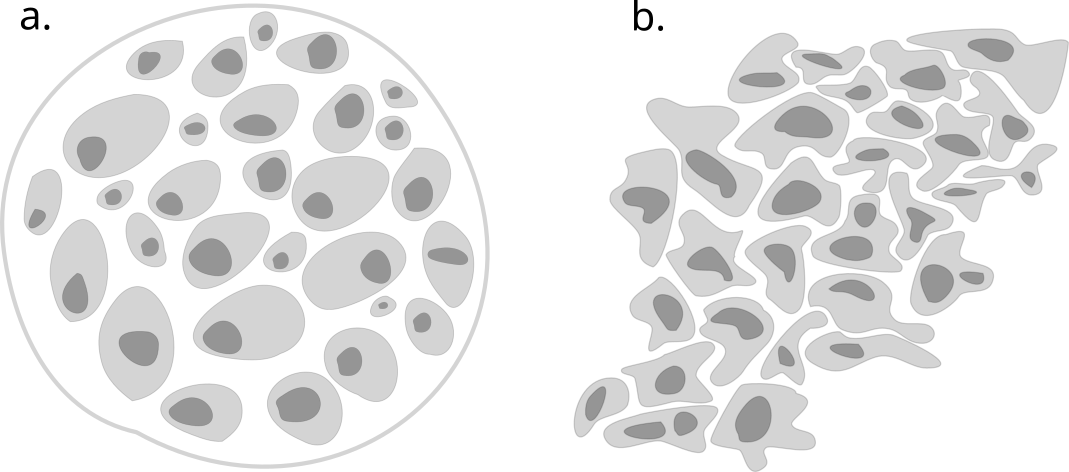
\includegraphics[scale=0.5]{KlasyfikacjaNowotworu.png}
\caption{Schematyczna ilustracja nowotworu łagodnego oraz złośliwego }
\end{figure}

Rysunek 2.1 przedstawia schematyczny wygląd:\\
a) nowotworu łagodnego, wyróżniającego się wyrażnie zaznaczoną torebką odgraniczającą komórki nowotworowe od zdrowych.\\
b) nowotworu złośliwego, charakteryzującego się nieregularną budowa oraz brakiem torebki, dzięki czemu może on naciskać na zdrowe tkanki co skutkuje jego rozrostem.\\

Do klasyfikacji  ze względu na typ tkanki z której się wywodzą zaliczamy:\\
\textbf{Nowotwory nabłonkowe} – nowotwory wywodzące się z tkanki nabłonkowej, złośliwe nowotwory nabłonkowe określane są pojęciem raka np. rak piersi, rak mózgu.\\
\textbf{Nowotwory nienabłonkowe} – nowotwory wywodzące się z tkanek innych niż nabłonek, ich nazwy tworzone są poprzez przekształcenie tkanki z której się wywodzą np. tłuszczak, mięśniak.\\


\section{Rozwój nowotworu (kancerogeneza)}
Nowotwory powstają w wyniku nieprawidłowego podziału komórek, którego powodem są uszkodzenia czy też mutacje zarówno pojedynczych genów jak i całego chromosomu. Proces przemiany komórki zdrowej w komórkę rakową nosi nazwę onkogenezy.
Skutkiem tych uszkodzeń jest utrata przez komórkę mechanizmów odpowiedzialnych za powstrzymanie jej podziału w razie uszkodzeń lub kontaktu z innymi komórkami (apoptoza) prowadząc do powstania tkanki nowotworowej [3, 4].\\
Kancerogeneza jest zazwyczaj procesem długotrwałym trwającym średnio 5 lat, ale może zajmować nawet powyżej 10 lat. W tym czasie powstaje guz nowotworowy o średnicy około 1cm, mogący zostać wykryty przy użyciu badań obrazowych takich jak USG.
Wyróżnia się 3 różne etapy kancerogenezy [3, 4]:\\
\textbf{1. Inicjacja} - w trakcie tego etapu pojawiają się pierwsze uszkodzenia DNA co prowadzi do procesu nowotworzenia. Jeśli uszkodzenia nie zostaną naprawione lub zaburzony zostanie proces apoptozy (przez co komórka nie obumrze) dochodzi do inicjacji procesu przemiany nowotworowej.\\
\textbf{2. Promocja} - podczas etapu promocji aktywowane są onkogeny (geny, których aktywność może prowadzić do mutacji nowotworowych), skutkiem czego dochodzi do intensywnego namnażania się uszkodzonych komórek. Wynikiem tego namnażania jest pojawienie się wielu nowych mutacji, wraz z postępem których zmiana nowotworowa staje się coraz groźniejsza. Etap ten może trwać wiele lat i skutkuje  przemianą zmutowanej komórki w komórkę nowotworową. Zmiany usunięte podczas tego etapu dają bardzo duże szansę na wyleczenie pacjenta.\\
\textbf{3. Progresja} – jest to ostatni etap kancerogenezy, w wyniku namnażania i różnicowania się komórek dochodzi do powstania guza nowotworowego oraz uzyskania zdolności naciekania i tworzenia przerzutów. Podczas tego etapu kariotyp (zestaw chromosomów komórki) ulega zmianom, a uszkodzenia komórki widoczne są pod mikroskopem.\\

\begin{figure}[h]
\centering
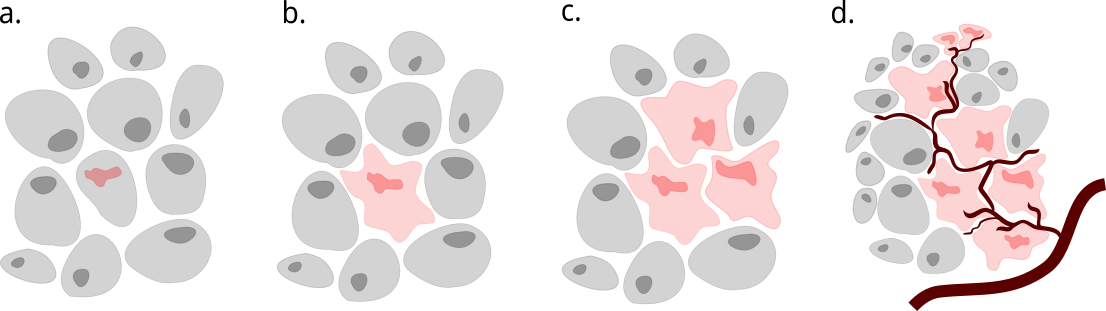
\includegraphics[scale=0.55]{SchematKancerogenezy.png}
\caption{Schemat kancerogenezy }
\end{figure}

Na rysunku 2.2 schematycznie pokazano kolejne etapy kancerogenezy począwszy od pierwszego uczkodzenia DNA (a), po widoczne rozprzestrzenianie się nowotworu na etapie promocji (b, c.) aż do powstania pełnego guza nowotworowego (d), wykazującego cechy anginogenezy co może skutkować przerzutami do odległych części ciała. 
Czynnikami powodującymi te uszkodzenia mogą być promieniowanie jonizujące, promieniowanie ultrafioletowe oraz wszystkie inne czynniki skutkujące długotrwałym drażnieniem tkanek, takie jak: konsumpcja alkoholu, nikotyna wraz z innymi substancjami zawartymi w dymie tytoniowym, pył azbestowy lub nawet długotrwała konsumpcja pikantnych potraw oraz poparzenia. Rak może też być wywołany przez wirusy onkogenne (onkowirusy).


\section{Leczenie chorób nowotworowych}
Popularnym przekonaniem jest to że, wykrycie choroby nowotworowej zawsze jest wyrokiem śmierci. Stwierdzenie to jest mylące gdyż, nowotwory które zostały wykryte u pacjenta we wczesnym stadium najczęściej prowadzą do całkowitego wyleczenia, nawet jeśli nowotwór zostanie wykryty w zaawansowanym stadium często możemy z nim bardzo długo żyć, jeśli tylko podejmiemy odpowiedni proces jego leczenia. Istnieje wiele sposobów walki z nowotworem, a sama onkologia jest jedną z najszybciej rozwijających się dziedzin medycyny.
Do technik standardowych zaliczamy [5, 6, 7]:\\
 \textbf{1. Operacja chirurgiczna} - jest jedną z najczęściej stosowanych technik leczenia, i w zależności od danej sytuacji może ona być zarówno połączona z innymi dostępnymi metodami jak i jedyną formą leczenia. Zazwyczaj polega ona na usunięciu tkanki nowotworowej wraz z częścią zdrowej tkanki ją otaczającej. Dzięki szybkiemu rozwoju onkologii coraz częściej wykonywane są operacje oszczędzające narząd dotknięty nowotworem, lub nawet operacje rekonstrukcyjne.\\
\textbf{2. Chemioterapia} – metoda polegająca na podawaniu pacjentowi leków hamujących proces podziału komórek nowotworowych (cytostatyków). Niestety leki te oddziaływują także na zdrowe szybko dzielące się komórki budujące różne tkanki naszego organizmu jak szpik kostny, nabłonek jelit lub naskórek co powoduje negatywne skutki uboczne jak wypadanie włosów, zapalenie błon śluzowych czy neurotoksyczność. Często stosowana jest w celu wspomagania innych metod leczenia i łagodzenia objawów nowotworu zaawansowanego.\\
\textbf{3. Radioterapia} – miejscowa metoda leczenia nowotworów złośliwych za pomocą promieniowania jonizującego. Promieniowanie to hamuje rozwój nowotworu poprzez uszkodzenie DNA komórek nowotworowych powodując utratę ich zdolności do podziału i zahamowanie jego rozwoju. Samą radioterapie można dalej podzielić ze względu na sposób napromieniowania na: brachyterapię oraz teleterapię. W brachyterapii źródło promieniowania umieszczane jest w obszarze tkanki nowotworowej za pomocą aplikatora zawierającego radioaktywny izotop. Wyróżnia się brachyterapię wewnątrztkankową, powierzchniową, wewnątrzjamową i śródoperacyjną. W teleterapii źródłem promieniowania jest urządzenie zewnętrzne. Teleterapia jest sposobem o wiele mniej inwazyjnym od brachyterapii w której aby umieścić źródło promieniowania w ciele pacjenta często należy zastosować znieczulenie ogólne.\\
\textbf{4. Immunoterapia} – jedna z najbardziej rewolucyjnych oraz szybko rozwijających się metod leczenia nowotworów. Polega na wzmocnieniu i wykorzystaniu systemu immunologicznego pacjenta w celu efektywniejszej walki z chorobą. Nawet u zdrowego człowieka system odpornościowy często ma trudności z poprawnym rozpoznaniem komórek rakowych czy to z powodu tego że nie są one wystarczająco „inne” od zdrowych komórek czy nawet w przypadku niektórych nowotworów, ich komórki mogą wytwarzać substancje mylące układ odpornościowy. Immunoterapię można podzielić na swoistą (przeciwciała monoklonalne i szczepionki antynowotworowe) oraz nieswoistą (cytokiny, monocyty, preparaty immunostymulujące i komórki LAK).\\
\textbf{5. Hormonoterapia} – ma na celu zaburzenie środowiska hormonalnego pacjentów hamując wzrost hormonozależnych nowotworów jak rak piersi. Metoda ta wykorzystuje jeden z mechanizmów: ablacyjny (ograniczenie lub całkowite zatrzymanie działania hormonu poprzez napromieniowanie lub całkowite usunięcie gruczołu czy też zastosowanie leków), addytywny (podanie hormonów zaburzających rozwój nowotworu), antagonistyczny (podanie leków blokujących receptory hormonów) oraz konkurencyjny czyli podanie leków wiążących się z receptorami co prowadzi do zmniejszenia wytwarzania lub oddziaływania hormonów płciowych na komórki docelowe. Jest to metoda tańsza oraz mniej inwazyjna od chemioterapii a więc lepiej nadaje się do leczenia paliatywnego (objawowego), niestety zajmuje więcej czasu oraz nie każdy chory może na nią pozytywnie zareagować.\\
\textbf{6. Terapia celowania} – jest to bardzo nowoczesne podejście wykorzystujące badania genetyczne wykonywane u chorego w celu stworzenia terapii dostosowanej do jego unikatowych potrzeb. Jest to bardzo precyzyjna terapia, atakująca tylko komórki nowotworowe w przeciwieństwie do chemioterapii która uszkadza zarówno komórki zdrowe jak i chore. Pomimo tego iż terapia celowana jest o wiele mniej toksyczna od chemioterapii, jest ona terapią długotrwałą przez co również może powodować niechciane skutki uboczne takie jak zapalenie skóry czy ogólne osłabienie, a to może prowadzić do decyzji o tymczasowym przerwaniu lub zakończeniu leczenia.\\





\chapter{Uczenie maszynowe}
Uczenie maszynowe to podzbiór szeroko pojętej Sztucznej Inteligencji - SI (ang. Artificial Intelligence) i nie należy tych pojęć mylić gdyż celem Sztucznej Inteligencji jest nadanie komputerom zdolności  imitowania ludzkiego zachowania, myślenia i wykonywania zadań.\\

\begin{figure}[h]
\centering
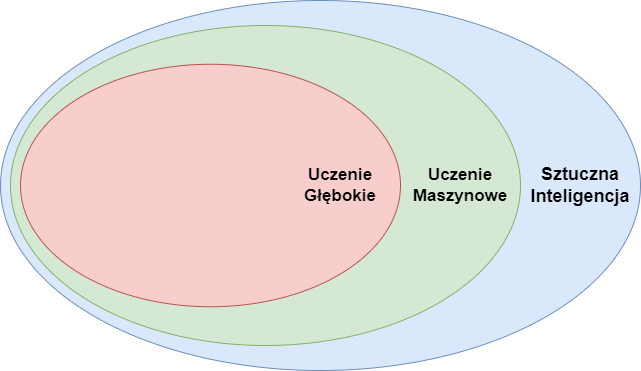
\includegraphics[scale=0.55]{UczenieMaszynowe.png}
\caption{Umiejscowienie uczenia maszynowego w ramach SI}
\end{figure}

Uczenie maszynowe natomiast koncentruje się na programowaniu komputerów w taki sposób aby posiadały one zdolność do samodzielnego uczenia się na podstawie przedstawionych im danych. Jedną z popularniejszych definicji uczenia maszynowego jest:\textit{„Field of study that gives computers the ability to learn without being explicitly programmed” („Dział nauki dający komputerom zdolność uczenia się bez bycia wprost zaprogramowanym”)} którą sformułował Arthur Samuel w 1959 roku [8]. Przykładami zastosowania uczenia maszynowego są m.in. filtry spamu, systemy rekomendacyjne, przewidywanie zachowań giełdy czy analiza genomu człowieka.  

\section{Uczenie maszynowe na przestrzeni lat}
Początki uczenia maszynowego jak i sztucznej inteligencji sięgają lat 40. i 50. ubiegłego wieku. Autorem pierwszego uczącego się programu był Arthur Samuel, przez wielu uważany za ojca uczenia maszynowego. Celem tego programu było nauczyć się grać w warcaby na takim poziomie aby „komputer” mógł stawić czoła przeciętnemu człowiekowi. Pierwszą jego wersję zaprezentował w 1952 r, w tym samym roku jako pierwszy użył on pojęcia „uczenie maszynowe”. Pierwszą uczącą się wersję systemu ukończył w 1955 r. Została ona zaprezentowana w telewizji w 1956 r. Kolejnym ważnym wynalazkiem w zakresie sztucznej inteligencji a zwłaszcza uczenia maszynowego był perceptron, wynaleziony przez Franka Rosenblatta [9]. Początkowo perceptron miał być maszyną a nie programem a jego pierwotną implementacją była maszyna nazwana Mark 1 perceptron, której zadaniem było rozpoznawanie znaków alfanumerycznych. Uważa się ją za pierwszy neurokomputer. Wraz z wynalezieniem perceptronu odkryty został fakt, że wykorzystanie wielu warstw perceptronów znacznie zwiększało jego możliwości. Skutkiem tego odkrycia było powstanie pierwszych jednokierunkowych sieci neuronowych (ang. feedforward neural network) oraz propagacji wstecznej (ang. backpropagation) [10]. Propagacja wsteczna umożliwia sieci dostosowanie swoich ukrytych warstw tak aby lepiej radziła sobie z nowymi przypadkami, jest ona obecnie używana to trenowania wszelkich sieci neuronowych. W roku 1967 za sprawą opracowania algorytmu K-najbliższych sąsiadów (ang. K-nearest neighbors, KNN) otworzyło się nowe pole badawcze w obrębie uczenia maszynowego, mianowicie rozpoznawanie wzorców czyli wykrywanie i grupowanie danych na podstawie ich wspólnych cech i zależności. Na przełomie lat 70. i 80. ubiegłego wieku uczenie maszynowe skupiło się na rozwijaniu sieci neuronowych lecz dotknęła je stagnacja, a sama sztuczna inteligencja skupiła się na wykorzystaniu modeli opartych o wiedzę, zamiast algorytmów przez co uczenie maszynowe stało się oddzielną dziedziną wiedzy. 
Bardziej dynamiczny rozwój statystycznego uczenia maszynowego nastąpił w latach 80. i 90. dzięki badaniom  Leo Breinmana z Uniwersytetu Kalifornijskiego w Berkley oraz Jerrego Freidmana z Uniwersytetu Stanforda. W 1984 roku Breinman wraz z swym zespołem stworzył drzewa decyzyjne - jedną z popularniejszych metod zarówno klasyfikacji jak i regresji [11]. Dekadę później opisał kolejną z przełomowych metod uczenia zagregowanego, którą jest bagging (ang. bootstrap aggregation), co doprowadziło do powstania lasów losowych (ang. Random Forests) czyli wykorzystania baggingu w drzewach decyzyjnych. Drugim istotnym osiągnięciem w zakresie statystycznego uczenia maszynowego był boosting, zaprezentowany przez Roberta Schapierea w artykule pt.  „The strength of weak learnability” (Siła słabego nauczania) [12].  Boosting, bagging oraz lasy losowe dały podstawy statystycznego uczenia maszynowego. W latach 90. a dokładniej w 1997 roku opracowana została technika głębokiego uczenia LSTM (ang. Long Short-Term Memory), która dziś wykorzystywana jest w dziedzinie rozpoznawania mowy. Jej autorami byli Jürgen Schmidhuber  i Sepp Hochreiter [13].   Efektem eksplozji internetu na początku XXI wieku był dostęp do nieporównywalnie większej ilości danych, które można było wykorzystać do trenowania wszelakich modeli uczenia maszynowego. Dzięki temu powstało przekonanie, że ilość i jakość danych jest tak samo ważna jak sam model. Wraz z rozwojem technik głębokiego uczenia, wielkie postępy zostały poczynione w dziedzinie rozpoznawania obrazów np. algorytm DeepFace stworzony przez Facebook (obecnie Meta), który potrafi rozpoznawać twarze na poziomie równym człowiekowi. Obecnie uczenie maszynowe jest jedną z najszybciej rozwijających się dziedzin Sztucznej Inteligencji, wykorzystywane jest w systemach rekomendacyjnych, aż po tworzenie autonomicznych samochodów a kończąc na analizie genomu. Ponadto dzięki temu że wiele technik uczenia maszynowego wykorzystywanych jest w analizie danych, często skutkuje to szybszym rozwojem dziedziny w której elementy uczenia maszynowego są stosowane, np. biocybernetyka czy medycyna.

\section{Typy uczenia maszynowego}
W uczeniu maszynowym (podobnie jak w każdej dziedzinie) istnieje wiele sposobów rozwiązywania danego problemu. Wybór typu uczenia maszynowego zależny jest w głównej mierze od zbioru danych z których ma nasz model korzystać. Algorytmy uczenia maszynowego można przyporządkować do trzech głównych grup [14, 15]:\\
\textbf{Uczenie nadzorowane}\\
      W przypadku uczenia nadzorowanego (ang. supervised learning)  model uczy się na podstawie danych mu przykładów z odpowiedzią. W przypadku problemu klasyfikacji (ang. classification) zbiór danych wykorzystywany przez model zawiera etykiety (ang. labels),  zaś w przypadku problemu regresji (ang. regression) – liczby rzeczywiste. Zbiór uczący z którego korzystają algorytmy uczenia nadzorowanego przyjmuje postać $(x, y)$, gdzie $x$ jest zbiorem wektorów przykładów uczących, zaś y to zbiór etykiet lub liczb im przypisanych. Algorytm w fazie uczenia ma za zadanie znaleźć funkcję $f\left(x_i\right)=y_i$ gdzie $i$ oznacza numer elementu ze zbioru uczącego. Znalezienie tej funkcji pozwala algorytmowi na przydzielenie odpowiedniej etykiety lub liczby dla danego przykładu. Do algorytmów uczenia nadzorowanego należą m.in. regresja liniowa i logistyczna, maszyny wektorów wsparcia (ang. support vector machines), K-najbliższych sąsiadów (K – nearest neighbors), drzewa decyzyjne i  lasy losowe. \\

\textbf{Uczenie nienadzorowane}\\
      Jak sama nazwa wskazuje zbiór danych wykorzystywany do zadań uczenia nienadzorowanego (ang. unsupervised learning) nie posiada etykiet, lub wartości które algorytm ma przewidywać, a więc sam zbiór przyjmuje postać $(x)$. Zamiast tego zadaniem algorytmów uczenia nienadzorowanego jest znalezienie wzorców i zależności w danych oraz ich pogrupowanie. Uczenie nienadzorowane może rozwiązywać o wiele bardziej skomplikowane problemy niż uczenie nadzorowane, jednakże będąc o wiele bardziej nieprzewidywalne może prowadzić do nieoczekiwanych lub nawet niechcianych efektów. Do algorytmów uczenia nienadzorowanego zaliczamy m.in. analizę danych składowych (ang. principal component analysis, PCA), grupowanie k-średnich, grupowanie hierarchiczne i  DBSCAN.\\

\textbf{Uczenie częściowo nadzorowane}\\
      Jest to metoda uczenia w przypadku której zbiór treningowy wygląda podobnie jak dla  uczenia nadzorowanego z dodatkiem przykładów nie posiadających żadnej etykiety lub wartości. Metodę tę można uznać za swoiste połączenie uczenia nadzorowanego z nienadzorowanym. Popularnym algorytmem stosowanym w uczenie częściowo nadzorowanym jest algorytm propagacji etykiet (ang. label propagation algorithm). Innym popularnym algorytmem uczenia częściowo nadzorowanego są generatywne sieci przeciwników (ang. generative adversarial networks, GAN).\\

\textbf{Uczenie przez wzmacnianie}\\
      Uczenie przez wzmacniane (ang. reinforcement learning)  znacznie różni się od pozostałych typów uczenia maszynowego. Poprzednio wspomniane algorytmy zawsze korzystały ze zbiorów danych na podstawie których miały określić pewne wartości lub znaleźć w nich zależności. W uczeniu przez wzmacnianie nie występuje jako taki zbiór danych, jego rolę pełni tzw. środowisko w którym porusza się nasz algorytm, potocznie agent. Agent ma za zadanie osiągnąć konkretny cel np. nauczyć się grać, a raczej wygrać w grę. Wszelkie akcje podejmowane przez algorytm są oceniane pozytywnie lub negatywnie na podstawie tego czy prowadzą do osiągnięcia celu i jak bardzo są efektywne. Zatem samym celem algorytmu jest maksymalizacja tych ocen, lub wzmocnień aby osiągnąć cel w jak najbardziej optymalny sposób. Podstawami uczenia przez wzmacnianie były procesy decyzyjne Markowa. Algorytmami uczenia przez wzmacnianie są m.in. algorytmy Monte Carlo, Q-Learning czy state–action–reward–state–action  (SARSA).\\

\section{Statystyczne uczenie maszynowe}
Statystyka i uczenie maszynowe od zawsze były ze sobą ściśle powiązane, wiele z metod uczenia maszynowego jest niczym innym jak modelami statystycznymi jak np. regresja liniowa czy logistyczna przez co nie istnieje ściśle określona granica między statystyką (dokładniej modelowaniem predykcyjnym) a samym uczeniem maszynowym. Można powiedzieć że największą różnicą między statystyką a uczeniem maszynowym jest ich cel, gdzie statystyka skłania się bardziej ku teorii prawdopodobieństwa i samej budowie danego modelu podczas gdy uczenie maszynowe skupia się na rozwoju efektywnych modelów, optymalizując je pod kątem wielkich zbiorów danych oraz poprawności predykcji, która w przypadku statystyki jest często drugorzędna.
\subsection{Bagging i lasy losowe}
\textbf{Bagging} (ang. bootstrap aggregating) jest jednym z dwóch modeli uczenia zagregowanego, czyli takiego w którym końcowy wynik (predykcje) otrzymujemy poprzez głosowanie większościowe lub uśrednienie predykcji wielu modeli [14]. Metoda ta niewiele różni się od zwyczajnego algorytmu agregacji, jedyną różnicą jest to iż w przypadku baggingu każdy nowy model zamiast korzystać z tego samego zbioru danych, korzysta z nowej próby bootstrapowej. Zbiór bootstrapowy zostaje stworzony przez losowe wybranie ze zwracaniem (elementy mogą się powtarzać) elementów ze zbioru treningowego. Elementy nie wylosowane podczas próby tworzą tzw. zbiór „out-of-bag” (poza workiem).\\
Przybliżony opis algorytmu baggingu wygląda następująco:\\
1. Stwórz $n$ zbiorów bootstrapowych.\\
2. Dla każdego ze zbiorów dopasuj oddzielny model predykcyjny.\\
3. Wykorzystaj wytrenowane klasyfikatory do predykcji nowych rekordów.\\
4. Określ końcową predykcję na podstawie wybranej metody np. uśrednienia lub wyboru większości.\\
Poniżej zaprezentowano wzory przykładowych metod liczenia ostatecznego wyniku.\\
W przypadku regresji, można wykorzystać średnią arytmetyczną, gdzie:\\
\noindent $F\left(x\right)\ $ - końcowy wynik dla rekordu $x$ ze zbioru testowego.\\
\noindent $f_n\left(x\right)\ $ - wynik $n$-tego modelu wytrenowanego na $n$-tym zbiorze danych dla rekordu $x$ :\\
\noindent
\begin{equation}
F\left(x\right)=\frac{\sum^N_{n=1}{f_n(x_n)}}{N}.
\end{equation}
W przypadku klasyfikacji natomiast możemy posłużyć się „głosowaniem większościowym”:\\
- dominanta (potocznie moda) wskazuje najczęściej występującą wartość w danym zbiorze
\noindent
\begin{equation}
F\left(x\right)=mode\left(f_1\left(x\right),\ f_2\left(x\right),\ \dots ,\ f_N\left(x\right)\right).
\end{equation}
\textbf{Lasy losowe} (ang. random forests) to zastosowanie metody baggingu dla modelu drzewa decyzyjnego. Między tymi podejściami istnieje jednak zasadnicza różnica: w lasach losowym poza próbkowaniem rekordów, próbkuje się również same zmienne. Zmienne próbkowane mogą być losowo (bez zwracania) lub wykorzystując miary zanieczyszczenia lub homogeniczności węzła. Do najpopularniejszych metod szacowania tychże miar należą miara Giniego zanieczyszczenia węzła (ang. Gini impurity) określona wzorem [14]:\\
\noindent
\begin{equation}
Gini\left(x\right)=1-\sum^j_{i=1}{p^2_i}
\end{equation}
$Gini(x)$ - miara zanieczyszczenia węzła $x$. \newline
\noindent $p_i$ - prawdopodobieństwo wylosowania klasy i w danym węźle.\\
oraz Entropia Informacji (ang. Entropy of Information) określona wzorem [14]:
\noindent
\begin{equation}
E\left(x\right)=\ -\sum^j_{i=1}{p_i{{\mathrm{log}}_2 p_i\ }}
\end{equation}
W ten sposób możemy określić atrybuty zbioru danych najlepiej go rozdzielające. Dzięki temu lasy losowe jak i same drzewa decyzyjne mogą zostać wykorzystane również w celu selekcji cech (ang. feature selection). Istotność zmiennej można również badać mierząc miarę spadku dokładności modelu wykorzystując do tego zbiór out-of-bag, można to porównać do swoistej walidacji krzyżowej.\\

\begin{figure}[h]
\centering
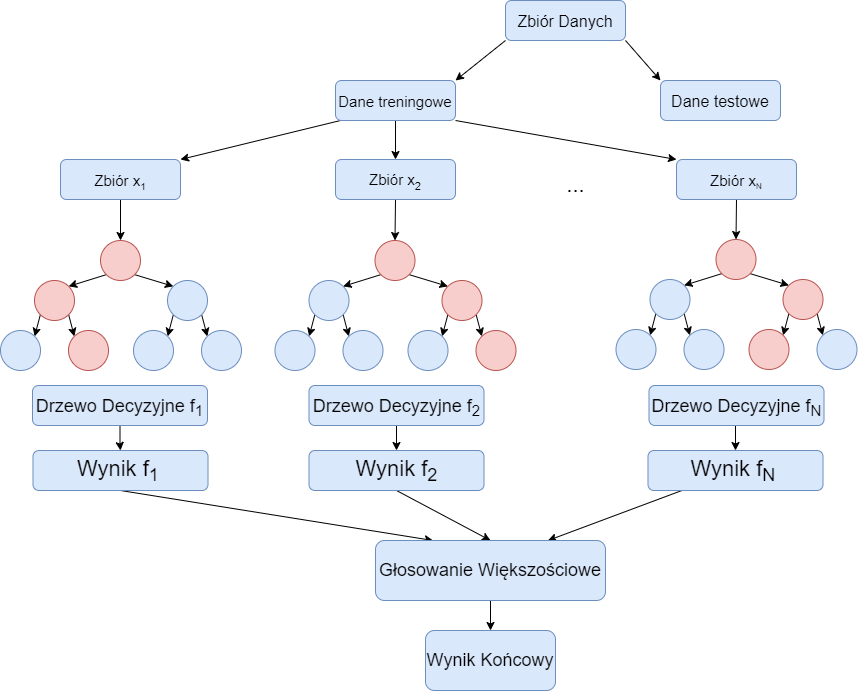
\includegraphics[scale=0.45]{RandForest.png}
\caption{Schemat modelu lasu losowego }
\end{figure}

Przez wykorzystanie wielu drzew (często setek lub tysięcy) lasy losowe są metodą „czarnej skrzynki”, oznacza to, że w przeciwieństwie do pojedynczego drzewa decyzyjnego niemożliwe jest  określenie dokładnych reguł decyzyjnych na podstawie których dane zostają klasyfikowane.

\subsection{Boosting}
Drugą techniką uczenia zagregowanego jest boosting. Tak jak bagging wykorzystuje wiele modeli w celu stworzenia jednego silnego modelu, lecz gdzie w przypadku baggingu modele były od siebie niezależne oraz uczyły się równolegle, tak w boostingu proces uczenia jest sekwencyjny. Został on rozwinięty w tym samym czasie co bagging. Główną ideą boostingu jest sekwencyjne trenowanie modeli, gdzie każdy kolejny klasyfikator próbuje skorygować błędy popełniane przez jego przodka. Wynik pojedynczego klasyfikatora zwany jest \textit{słabą hipotezą} (ang. \textit{weak hypothesis}). Osiągane jest to przez zwiększanie początkowo przydzielonych wag rekordów, które zostały błędnie zaklasyfikowane przez model, oraz zmniejszanie wag rekordów zaklasyfikowanych poprawnie. Istnieje kilka wariantów boostingu. Do najpopularniejszych zaliczamy AdaBoost (ang. Adaptive Boosting), gradient boosting (wzmacnianie gradientowe) oraz stochastic gradient boosting (stochastyczne wzmacnianie gradientowe). Poniżej przedstawiono schemat działania AdaBoost dla zbioru danych $x=(x_1,y_1 ),…,(x_m,y_m )$ gdzie każde  $x_i$ należy do zbioru rekordów $X$, a $Y$ to zbiór etykiet odpowiadających tem rekordom, w tym przypadku $Y=\left\{-1,\ +1\right\}$ [17]:\\
Mając $m$ elementowy zbiór danych $x=\left(x_1,\ y_1\right),\dots ,\left(x_m,y_m\right)\ $gdzie $x_i\in X,\ y_i\in Y=\left\{-1,\ +1\right\}$\\
Zainicjalizuj $D_1\left(i\right)=1/m$ dla $i=1,\dots ,m$\\
Dla $t=1,\dots ,T$:

\begin{enumerate}
  \item Zbuduj słaby klasyfikator $h_t:X\to \{-1,\ +1\}$ uwzględniając rozkład $D_t$
  \item Oblicz błąd klasyfikatora dany wzorem:
  \begin{equation}
  e_t=\mathrm{P}{\mathrm{r}}_{i\sim D_t}[h_t(x_i)\neq y_i]   
  \end{equation}
  \item Oblicz wagę klasyfikatora ${\alpha }_t$ daną wzorem:
  \begin{equation}
  {\alpha }_t=\frac{1}{2}\mathrm{ln}\mathrm{}(\frac{1-e_t}{e_t})   
  \end{equation}

  \item Uaktualnij wagi elementów zbioru treningowego dla $i=1,\dots ,m$:
  \begin{equation}
   D_{t+1}\left(i\right)=\ \frac{D_t(i)\mathrm{exp}\mathrm{}(-{\alpha }_ty_ih_t\left(x_i\right))}{Z_t}    
  \end{equation}
\end{enumerate}

\noindent Gdzie $Z_t$ jest czynnikiem normalizującym dobranym tak aby $D_{t+1}$ było rozkładem\\
Oblicz finalną hipotezę opisaną wzorem:
\begin{equation}
 H\left(x\right)=sign\ \left(\sum^T_{t=1}{{\alpha }_th_t\left(x\right)}\right)   
\end{equation}


\newpage{}
\begin{figure}[h]
\centering
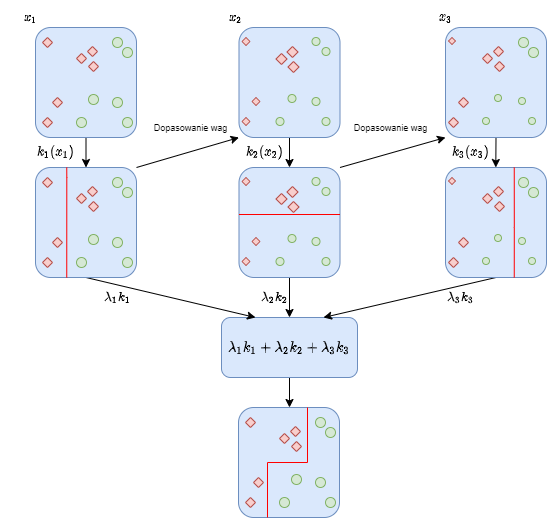
\includegraphics[scale=0.55]{Boosting.png}
\caption{Schemat działania metody boostingu}
\end{figure}


\subsection{Stacking}

Trzecią metodą uczenia zagregowanego jest stacking. Metoda ta w odróżnieniu od boosting i baggingu łączy wiele różnych modeli predykcyjnych takich jak drzewa decyzyjne, sieci neuronowe czy lasy losowe, które pełnią role modeli bazowych lub modeli poziomu pierwszego. Na podstawie wyników wskazywanych przez te modele tworzony zostaje zbiór treningowy, w którym cechami są predykcje tychże modeli. Otrzymany w ten sposób zbiór danych wykorzystywany jest do trenowania meta modelu lub modelu poziomu drugiego, który pełni funkcję ostatecznego predyktora. Funkcje meta modelu często pełnią proste, łatwo interpretowalne metody takie jak regresja liniowa w przypadku problemów regresji czy regresja logistyczna dla problemów klasyfikacji [18]. Zastosowanie stackingu nie zawsze jest związane z poprawieniem jakości modelu. Sama wydajność modelu mocno zależna jest od wyboru modeli bazowych, w najlepszym przypadku modele te czy też ich wyniki nie są ze sobą skorelowane. Naturalnie gdy jeden z modeli bazowych dorównuje wydajności stackingu należy posłużyć się nim ze względu na o wiele niższy stopień skomplikowania. Poniżej przedstawiono schemat działania metody stackingu dla N elementowego zbioru danych treningowych $X = {x_i,y_i}$ [19]:

\begin{enumerate}
  \item Wytrenuj n modeli bazowych od $f_1\dots f_n$ każdy na podstawie zbioru $X$
  \item Stwórz nowy $N$ elementowy zbiór danych $X^{'}=\left \{ x_{i}^{'},y_{i} \right \}$ na podstawie wyników modeli bazowych gdzie $x_{i}^{'}=\left\{f_1\left(x_i\right),\ f_2\left(x_i\right),\dots ,f_n\left(x_i\right)\right\}.$
  \item Wytrenuj meta model $f^{'}$  na bazie zbioru $X^{'}$.
  \item Zwróć model końcowy przyjmujący postać $F\left(x\right)=f^{'}\left(f_1\left(x\right),\ f_2\left(x\right)\dots f_n\left(x\right)\right).$
\end{enumerate}

\noindent Na rysunku 3.4 pokazano przykładowy schemat tej metody.

\begin{figure}[h]
\centering
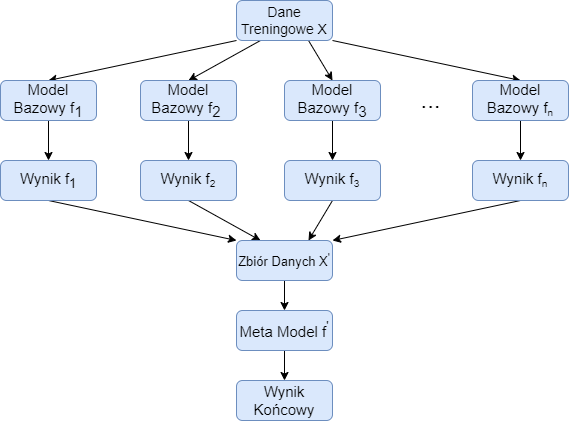
\includegraphics[scale=0.6]{Stacking.png}
\caption{Schemat metody stackingu}
\end{figure}



\subsection{K-najbliższych sąsiadów}
Algorytm K-najbliższych sąsiadów, KNN jest prostym i intuicyjnym algorytmem stosowanym zarówno w przypadku klasyfikacji jak i regresji. W skrócie polega on na przewidywaniu klasy (lub wartości) danego rekordu na podstawie określonej ilości (K) rekordów (sąsiadów) najbardziej do niego podobnych (najbliższych). Poziom podobieństwa rekordu określany jest za pomocą odległości do jego sąsiadów. Dwiema najpopularniejszymi funkcjami odległości są [20]:
\begin{enumerate}
    \item Odległość Euklidesowa (ang. Euclidean distance) określona jest równaniem:
    \begin{equation}
     d\left(x,\ y\right)=\sqrt{\sum^k_{i=1}{{\left(x_i-y_i\right)}^2}}   
    \end{equation}
    \item Odległość Manhattan (ang. Manhattan distance) dana jest wzorem:
    \begin{equation}
     d\left(x,y\right)=\sum^k_{i=1}{|x_i-y_i|}  
    \end{equation}
\end{enumerate}
Sam algorytm nie wymaga trenowania i jest bardzo prosty w implementacji oraz w samym zrozumieniu jego założenia, co nie oznacza że jego wykorzystanie jest procesem automatycznym i nie wymagającym wysiłku. Jakość wyników przez niego zwracanych zależy w dużej mierze od samego zbioru danych na którym operuje. Algorytm ten jest bardzo wrażliwy na zaszumione dane, wartości odstające jak i wartości brakujące. Sam zbiór danych trzeba poddać standaryzacji i normalizacji. Wybór ilości sąsiadów K nie jest banalny, gdyż nie istnieje „magiczna liczba” opisująca K. Należy jednak zwrócić uwagę, że istnieje kilka podstawowych zasad takich jak określanie K jako liczbę nieparzystą lub pierwiastek z liczby wszystkich rekordów w zbiorze danych. Poniżej przedstawiono schemat działania algorytmu KNN:
\begin{enumerate}
    \item Wybierz liczbę K sąsiadów.
    \item Oblicz daną metrykę odległości między klasyfikowanym rekordem a każdym z sąsiadów.
    \item Wybierz K najbliżej położonych sąsiadów.
    \item W przypadku klasyfikacji wybierz najliczniejszą klasę wśród sąsiadów, w przypadku regresji oblicz średnią wartość K najbliższych rekordów (sąsiadów).
\end{enumerate}

Na rysunku 3.5 zaprezentowano poglądową ilustracje działania algorytmu KNN.
\begin{figure}[h]
\centering
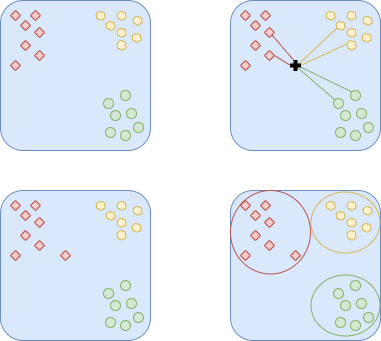
\includegraphics[scale=0.6]{KNN.png}
\caption{Poglądowa ilustracja działania algorytmu KNN}
\end{figure}


\chapter{Badania eksploracyjne zbioru danych oraz dopasowanie modeli}
Zbiorem będącym obiektem dalszych badań jest zbiór Breast Cancer Coimbra [21]. Zbiór ten zawiera dane 116 pacjentek z czego 64 są chore na raka piersi a pozostałe 52 to zdrowa grupa kontrolna. Każdy rekord zbioru posiada 10 cech, 9 badań wykonanych na pacjentce kolejno: wiek, BMI (wskaźnik masy ciała mierzony w $kg/m^{2}$), glucose (glukoza mierzona w $mg/dL$), insulin (insulina mierzona w $µU/mL$), HOMA (wskaźnik insulinoodporności), leptin (leptyna hormon sytości, mierzony w $ng/mL$), adiponectin (adiponektyna, mierzona w $µg/mL$), resistin (rezystyna, mierzona w $ng/mL$) i MCP-1 (białko chemotaktyczne monocytów, mierzone w $pg/dL$). Wyniki wszystkich badań oprócz wieku oraz BMI są uzyskiwane za pomocą analizy krwi. Ostatnią cechą jest diagnoza pacjentki, dopasowane modele będą miały za zadanie ją przewidzieć.
\section{Użyte narzędzia}
Do przeprowadzenia dalszych badań wykorzystany został język Python w środowisku Jupyter Notebook. Python jako wysokopoziomowy język ogólnego przeznaczenia, jest jednym z najpopularniejszych i najszybciej rozwijających się języków programowania. Zawdzięcza to w dużej mierze swojej prostej i przyjaznej składni, co powoduje że jest  jednym z najłatwiejszych języków do opanowania. Ponadto dysponuje znacznym zbiorem darmowych bibliotek pozwalających na tworzenie wszelakich aplikacji sieciowych, gier czy modeli uczenia maszynowego w bardzo krótkim czasie. W sferze sztucznej inteligencji oraz data science jest de facto językiem domyślnym. Badania wykonywane w dalszej części rozdziału będą wykorzystywać następujące biblioteki [22]:
\begin{enumerate}
    \item \textbf{Pandas} - najpopularniejsza biblioteka służąca do pracy z ustrukturyzowanymi danymi. Wprowadza strukturę „ramki danych” (ang. data frame) czyli tabelę w której wiersze i kolumny można opisywać etykietami oraz „seriami” (ang. series). Zawiera wiele zaawansowanych funkcji indeksowania, co zapewnia prostotę przetwarzania, dzielenia czy czyszczenia danych. Została ona stworzona w 2010 roku, a jej autorem jest Wes McKinney.
    \item \textbf{NumPy} - Numerical Python, podstawowa biblioteka do wykonywania obliczeń numerycznych. Wprowadza ona \textit{ndarray} - bardzo wydajny obiekt tablicowy, który często pełni funkcje przenośnika danych do np. modeli uczenia maszynowego. Sam pakiet Pandas został napisany przy użyciu funkcji biblioteki NumPy.
    \item \textbf{Plotly} – podobnie jak Matplotlib czy Seaborn pakiet ten służy do tworzenia wykresów i wizualizacji danych. Różni się od nich tym że każdy wykres jest interaktywny, bez potrzeby własnoręcznego programowanie tejże funkcjonalności, a sam wygląd wykresów jest na bardzo wysokim poziomie. Dodatkowo w połączeniu z pakietem \textit{Dash} można w bardzo prosty sposób tworzyć aplikacje sieciowe, które mogą działać nawet w trybie „inline” z notatnikiem Jupytera, czyli jako jego komórka.
    \item \textbf{Scikit-learn} – powstały w 2010 roku pakiet zawierający implementacje wszystkich obecnych modeli uczenia maszynowego, jak i metod ekstrakcji cech czy też selekcji modelu. Podobnie jak wszystkie poprzednie biblioteki jest on pakietem open-source przez co rozwija się w bardzo szybkim tempie. Jest on kolejnym z głównych powodów popularności Pythona w obszarze data science i uczenia maszynowego oraz samej sztucznej inteligencji.
    \item \textbf{Jupyter Notebook} – jest to interaktywny notes pozwalający na tworzenie kodu Markdown i HTML. Obsługuje on wiele języków i wykorzystywany jest do tworzenia interaktywnych notesów łączących tekst oraz kod czy nawet całych aplikacji sieciowych i jest bardzo szeroko wykorzystywany w dziedzinie data science. W serwisie Kaggle istnieją całe konkursy na najlepszy „notatnik” w których czasami można wygrać pokaźne nagrody pieniężne. Wszystko to prowadzi do tego że jest to jeden z najpopularniejszych formatów dzielenia się odkryciami i badaniami w zakresie data science i machine lerning.
\end{enumerate}
\section{Badania eksploracyjne}
Zawsze gdy w projekcie z zakresu uczenia maszynowego wykorzystywany jest obcy, nie znany zbiór danych bardzo dobrym pomysłem jest przeprowadzenie na nim badań eksploracyjnych (ang. Exploratory Data Analusis, EDA). Mają one na celu zobrazowanie własności zbioru danych za pomocą prostych wykresów takich jak np. histogramy czy wykresy punktowe, oraz statystyk podsumowujących (średnia, mediana, percentyle, itp.). Dzięki wykonaniu tychże badań często można przewidzieć jakie algorytmy (modele) będą najskuteczniejsze, lub czy do ich działania niezbędne będzie wykonanie określonych czynności takich jak usunięcie lub uzupełnienie brakujących wartości, redukcja wymiarowości, standaryzacja, normalizacja.
Wspomniany wcześniej Jupyter Notebook jest idealnym narzędziem w celu wykonania tego rodzaju badań i będzie wykorzystany w dalszej części tego rozdziału. Analizę nieznanego zbioru danych zawsze dobrze jest zacząć od sprawdzenia czy występują w nim jakieś wartości brakujące. Dzięki połączeniu funkcji \textit{DataFrame.isnull} oraz \textit{DataFrame.sum} poniższy kod umożliwia wyświetlenie tabeli zawierającej sumy wartości brakujących poszczególnej kolumny (jeśli takowe istnieją).

\begin{lstlisting}[language=Python, caption=Sumawanie wartości NaN]
df = pd.read_csv('BreastCancerCoimbra.csv')
df.isnull().sum()
\end{lstlisting}



 Zbiór danych nie zawiera żadnych wartości brakujących, ale nazwy wszystkich kolumn są w języku angielskim. Ze względu na przejrzystość zostaną one zamienione na język polski, oraz wartości kolumny „Classification” zamienione zostaną z numerycznych na kategorialne (Zdrowa, Chora), ponadto dodana zostanie nowa kolumna „Przedział Wiekowy”. Poniższy kod wykonuje te czynności:

\begin{lstlisting}[language=Python, caption=Dodawanie nowej cechy]
df['Classification'].replace({1: 'Zdrowa', 2: "Chora"}, inplace=True)
df['PrzedzialWiekowy'] = np.NaN
df['PrzedzialWiekowy'] = df.apply(lambda x:'Do 30 lat' if (x['Age'] <= 30)else '31-50 lat' if (x['Age'] > 30) and (x['Age'] <= 50)else 'Powyzej 50lat', axis=1)
df = df.rename(columns = {'Age': 'Wiek', 'Glucose': 'Glukoza', 'Insulin': 'Insulina','Leptin': 'Leptyna','Adiponectin': 'Adiponektyna','Resistin': 'Rezystyna','MCP-1': 'Bialko chemotaktyczne monocytow','Classification': 'Klasyfikacja'}, inplace = False)
\end{lstlisting}

Kolejną bardzo pomocną funkcją pakietu Pandas jest $DataFrame.describe$, pozwala ona na szybkie zbadanie elementów podsumowujących zbioru danych. Za pomocą kolejnej funkcji $Dataframe.astype$ możemy przekonwertować ramkę danych do wymaganego typu, w naszym przypadku będzie to typ całkowity int. Kolejną kluczową funkcją jest $DataFrame.loc$ pozwalająca na dostęp do grup rekordów na podstawie ich wartości.

\begin{lstlisting}[language=Python, caption=Wykorzystanie funkcji \textit{DataFrame.loc}]
display(df.loc[lambda df: df['Klasyfikacja'] == 'Zdrowa'].describe().astype(int))
display(df.loc[lambda df: df['Klasyfikacja'] == 'Chora'].describe().astype(int))
\end{lstlisting}

\begin{center}
\scalebox{0.85}{
\begin{tabular}{||c c c c c c c c c c||} 
 \hline
  & Wiek & BMI & Glukoza & Insulina & HOMA & Leptyna & Adiponektyna & Rezystyna & MCP.1 \\ [0.5ex] 
 \hline\hline
 count & 52 & 52 & 52 & 52 & 52 & 52 & 52 & 52 & 52 \\ 
 \hline
 mean & 58 & 28 & 88 & 6 & 1 & 26 & 10 & 11 & 499  \\
 \hline
 std & 18 & 5 & 10 & 4 & 1 & 19 & 7 & 11 & 292  \\
 \hline
 min & 24 & 18 & 60 & 2 & 0 & 4 & 2 & 3 & 45  \\
  \hline
 25\% & 41 & 23 & 82 & 4 & 0 & 11 & 5 & 6 & 260  \\
  \hline
 50\% & 65 & 27 & 87 & 5 & 1 & 21 & 8 & 8 & 471  \\
  \hline
 75\% & 75 & 32 & 93 & 7 & 1 & 36 & 10 & 12 & 642  \\
 \hline
 max & 89 & 38 & 118 & 26 & 7 & 83 & 38 & 82 & 1256  \\ [1ex] 
 \hline
\end{tabular}}
\end{center}

\begin{center}
\scalebox{0.85}{
\begin{tabular}{||c c c c c c c c c c||} 
 \hline
  & Wiek & BMI & Glukoza & Insulina & HOMA & Leptyna & Adiponektyna & Rezystyna & MCP.1 \\ [0.5ex] 
 \hline\hline
 count & 64 & 64 & 64 & 64 & 64 & 64 & 64 & 64 & 64 \\ 
 \hline
 mean & 56 & 26 & 105 & 12 & 3 & 26 & 10 & 17 & 563  \\
 \hline
 std & 13 & 4 & 26 & 12 & 4 & 19 & 6 & 12 & 384  \\
 \hline
 min & 34 & 18 & 70 & 2 & 0 & 6 & 1 & 3 & 90  \\
  \hline
 25\% & 45 & 22 & 92 & 4 & 1 & 12 & 5 & 8 & 299  \\
  \hline
 50\% & 53 & 27 & 98 & 7 & 2 & 18 & 8 & 12 & 465  \\
  \hline
 75\% & 68 & 30 & 109 & 16 & 4 & 37 & 12 & 22 & 737  \\
 \hline
 max & 86 & 37 & 201 & 58 & 25 & 90 & 33 & 55 & 1698  \\ [1ex] 
 \hline
\end{tabular}}
\end{center}

W wyniku wyświetlone zostały dwie tabele zawierające informacje o ilości rekordów, średniej, odchyleniu standardowym, wartości minimalnej i maksymalnej oraz kolejnych percentylach dla poszczególnych cech. Następna część badań skupiać się będzie na wykresach, do których stworzenia wykorzystana zostanie wspomniana wcześniej biblioteka Plotly. Pierwszym z nich jest histogram czyli wykres na którym na osi x ukazane są przedziały lub kategorie, zaś na osi y ich liczebności. Zaprezentowany histogram pokazuje relację pomiędzy ilością pacjentek ich przedziałem wiekowym oraz klasyfikacją, jest on przedstawiony poniżej wraz z odpowiadającym kodem: 

\begin{lstlisting}[language=Python, caption=Tworzenie histogramu]
px.histogram(df, x='Klasyfikacja', color='PrzedzialWiekowy', height=400, width=800)
\end{lstlisting}

\begin{figure}[H]
\centering
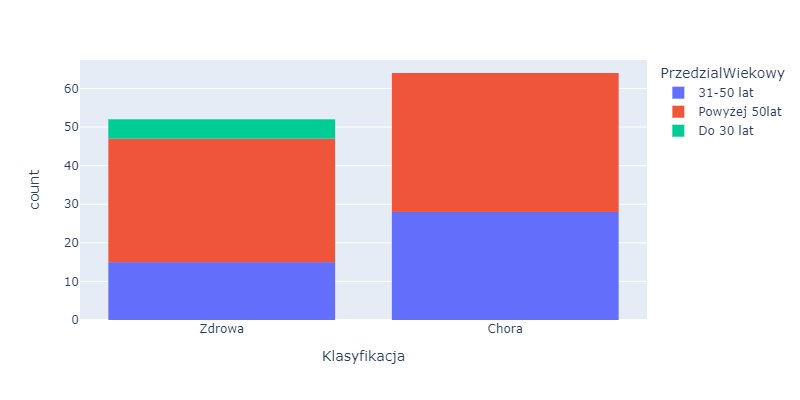
\includegraphics[scale=0.3]{pxhistoshow.png}
\caption{Relacje pomiędzy ilością pacjentek ich przedziałem wiekowym oraz klasyfikacją }
\end{figure}

Wykres z rys. 4.1 pokazuje że jest zdecydowanie więcej pacjentek chorych w wieku średnim, i co ciekawe ilość pacjentek zdrowych w wieku powyżej 50 lat jest bardzo podobna do ilości chorych (32 do 36). Biblioteka Plotly umożliwia również łatwe łączenie histogramów z wykresami konturowymi. Wykresy te wykorzystują kontury do zobrazowania związków między dwiema zmiennymi numerycznymi, są wyjątkowo przydatne gdy zbiór danych zawiera zbyt wiele rekordów aby wykres punktowy był czytelny. Wykres z rysunku 4.2 przedstawia zależność między poziomami glukozy a insuliny w poszczególnych grupach wiekowych pacjentek i podziałem ze względu na klasyfikacje.

\begin{lstlisting}[language=Python, caption=Tworzenie wykresu konturowego]
px.density_contour(df, x="Glukoza", y="Insulina", facet_col="PrzedzialWiekowy", color="Klasyfikacja", marginal_x="histogram", height = 600, width = 1000)
\end{lstlisting}

\begin{figure}[h]
\centering
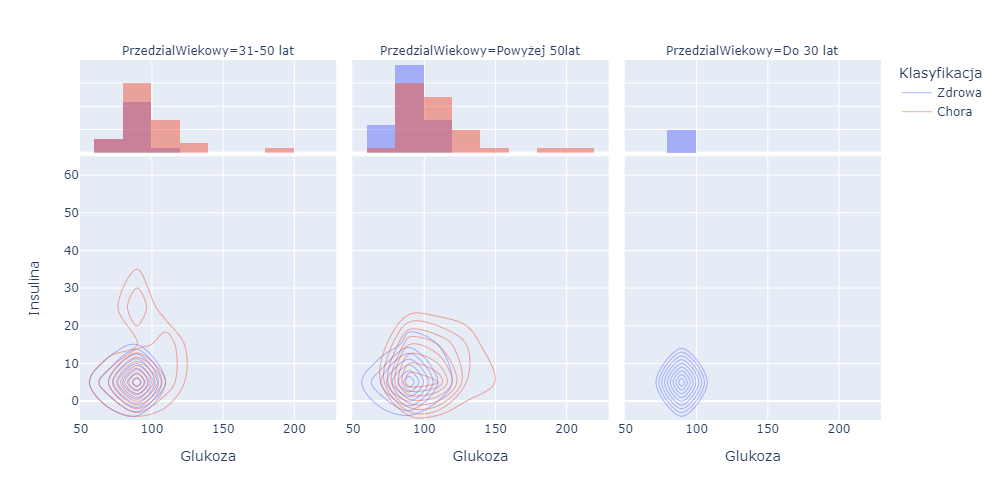
\includegraphics[scale=0.4]{pxdenscontshow.png}
\caption{Zależności między poziomami glukozy a insuliny w poszczególnych grupach wiekowych pacjentek}
\end{figure}

Następnymi dwoma wykresami, bardzo przydatnymi w przypadku pracy ze zbiorami zawierającymi zarówno dane kategorialne jak i numeryczne są wykresy pudełkowe (ang. boxplot) oraz ich rozszerzone wersje, tzw. wykresy skrzypcowe (ang. violin plot). Poniżej, odpowiednio na rysunkach 4.3 oraz 4.4 przedstawione obydwa te wykresy, operujące na tych samych danych w celu zobrazowania ich różnic, oraz kod je generujący, w przypadku wykresów skrzypcowych funkcje \textit{go.Box} wystarczy zamienić na \textit{go.Violin}.


\begin{lstlisting}[language=Python, caption=Tworzenie wykresu pudełkowego]
fig1 = make_subplots(rows = 1, cols = 4, shared_yaxes=False)
fig1.add_trace(go.Box(x = df['Klasyfikacja'], y = df['BMI'], name = 'BMI'),row = 1, col = 1)
fig1.add_trace(go.Box(x = df['Klasyfikacja'], y = df['Insulina'], name = 'Insulina'),row = 1, col = 2)
fig1.add_trace(go.Box(x = df['Klasyfikacja'], y = df['Glukoza'], name = 'Glukoza'),row = 1, col = 3)
fig1.add_trace(go.Box(x = df['Klasyfikacja'], y = df['Leptyna'], name = 'Leptyna'),row = 1, col = 4)
fig1.update_layout(height = 400, width = 800)
\end{lstlisting}



\begin{figure}[h]
\centering
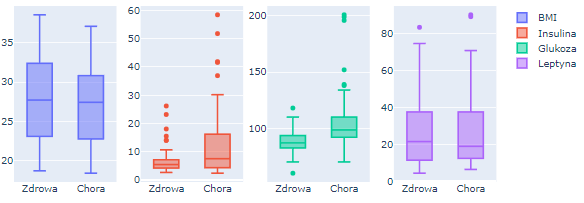
\includegraphics[scale=0.9]{pxboxshow.png}
\caption{Przykład wykresu pudełkowego }
\end{figure}

\begin{figure}[h]
\centering
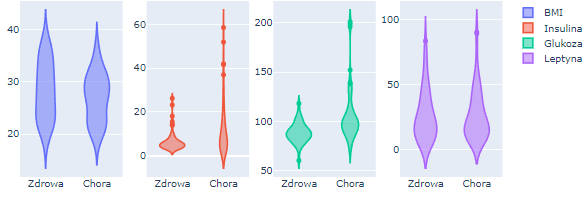
\includegraphics[scale=0.9]{pxviolinshow.png}
\caption{Przykład wykresu skrzypcowego }
\end{figure}

Główną różnicą między tymi wykresami jest to, że podczas gdy wykres pudełkowy wyraźnie pokazuje takie wartości jak mediana, kwartyle, oraz wartości graniczne wraz z odstającymi, wykres skrzypcowy natomiast operuje na funkcjach gęstości, pozwalając na ukazanie różnic rozkładu różnych zmiennych, niezauważalnych w przypadku wykresu pudełkowego. W przypadku biblioteki Plotly wartości odstające zaznaczone są również na wykresie skrzypcowym. Kolejnymi wykresami wykorzystanymi w EDA będą wykresy punktowe zarówno dwu jak i trójwymiarowe oraz wykres dywanowy. Wykresy punktowe rozmieszczają rekordy zbioru danych na płaszczyźnie kartezjańskiej, zazwyczaj dwuwymiarowej, najczęściej wykorzystywane w nich są dane numeryczne, lecz możliwe jest też wykorzystanie danych kategorialnych do dalszego rozróżnienia rekordów. Poniżej, na rys. 4.5 został przedstawiony dwuwymiarowy wykres punktowy wraz z dodatkowym wykresem dywanowym oraz kod go generujący.
Punkty na rysunku 4.5 rozmieszczone są na płaszczyźnie względem wartości poziomów insuliny oraz glukozy pacjentek. Kolorowi punktów odpowiada klasyfikacja (osoba zdrowa/chora) a wielkości wiek danej pacjentki. Na rys. 4.6 przedstawiony jest ten sam wykres z dodatkiem trzeciego wymiaru którym będzie BMI pacjentki.


\begin{lstlisting}[language=Python, caption=Tworzenie wykresu punktowego 2D]
px.scatter(df, x='Insulina', y='Glukoza', color='Klasyfikacja', symbol='Klasyfikacja', marginal_x="rug", size='Wiek', size_max=8, height = 500, width = 800)
\end{lstlisting}

\begin{figure}[H]
\centering
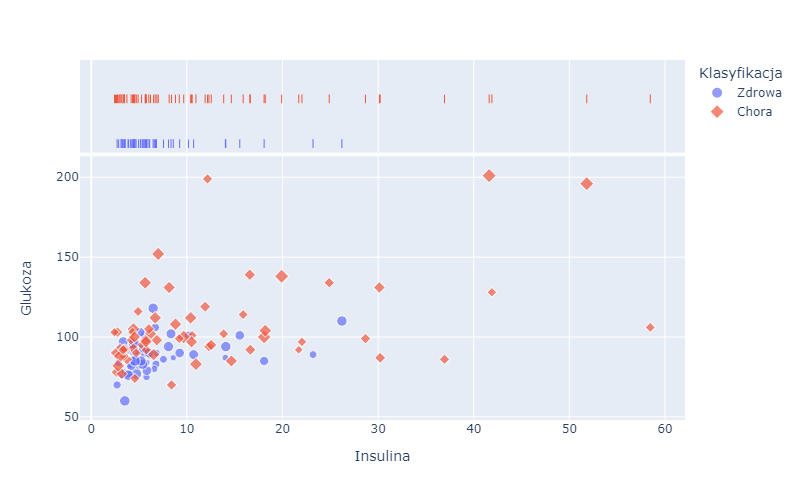
\includegraphics[scale=0.4]{2dNOCODE.png}
\caption{Dwuwymiarowy wykres punktowy }
\end{figure}

\begin{lstlisting}[language=Python, caption=Tworzenie wykresu punktowego 3D]
px.scatter_3d(df, x='Insulina', y='Glukoza', z='BMI' ,color='Klasyfikacja', symbol='Klasyfikacja', size='Wiek', size_max=12, opacity=0.8,  height = 500, width = 800)
\end{lstlisting}

\begin{figure}[H]
\centering
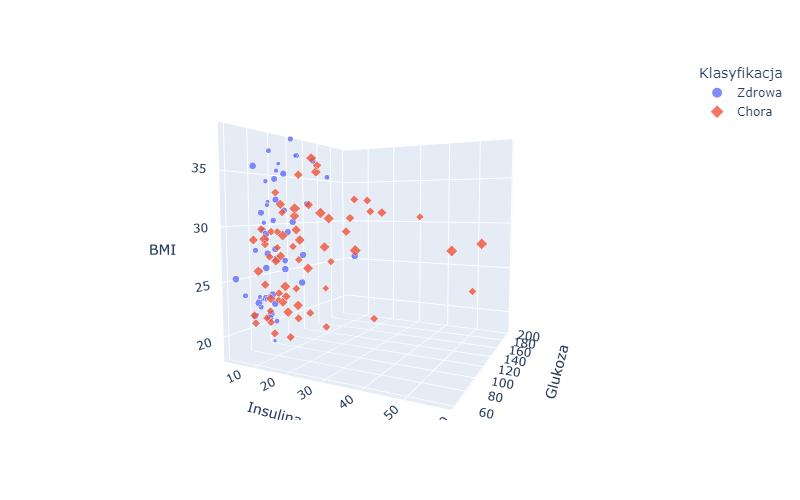
\includegraphics[scale=0.4]{3dNOCODE.png}
\caption{Trójwymiarowy wykres punktowy}
\end{figure}



Ostatnim wykresem użytym w procesie badań eksploracyjnych będzie mapa cieplna (ang. heatmap). Wykres ten obrazuje korelację pomiędzy każdym z atrybutów zbioru co jest bardzo przydatne podczas procesu redukcji wymiarowości zbioru. Wykres oraz kod go generujący pokazany jest na rysunku 4.7.


\begin{lstlisting}[language=Python, caption=Tworzenie mapy cieplnej]
mask = np.triu(np.ones_like(df.corr(), dtype=bool))
fig = go.Figure(data=go.Heatmap(z = df.corr().mask(mask), x = df.corr().columns, y = df.corr().columns, showscale=True, ygap=1, xgap=1))
fig.update_xaxes(side="bottom")
fig.update_layout(title_text='Mapa Cieplna', title_x=0.5, width=620, height=620, xaxis_showgrid=False, yaxis_showgrid=False, xaxis_zeroline=False, yaxis_zeroline=False, yaxis_autorange='reversed', template='plotly_white')
fig.show()
\end{lstlisting}

\begin{figure}[h]
\centering
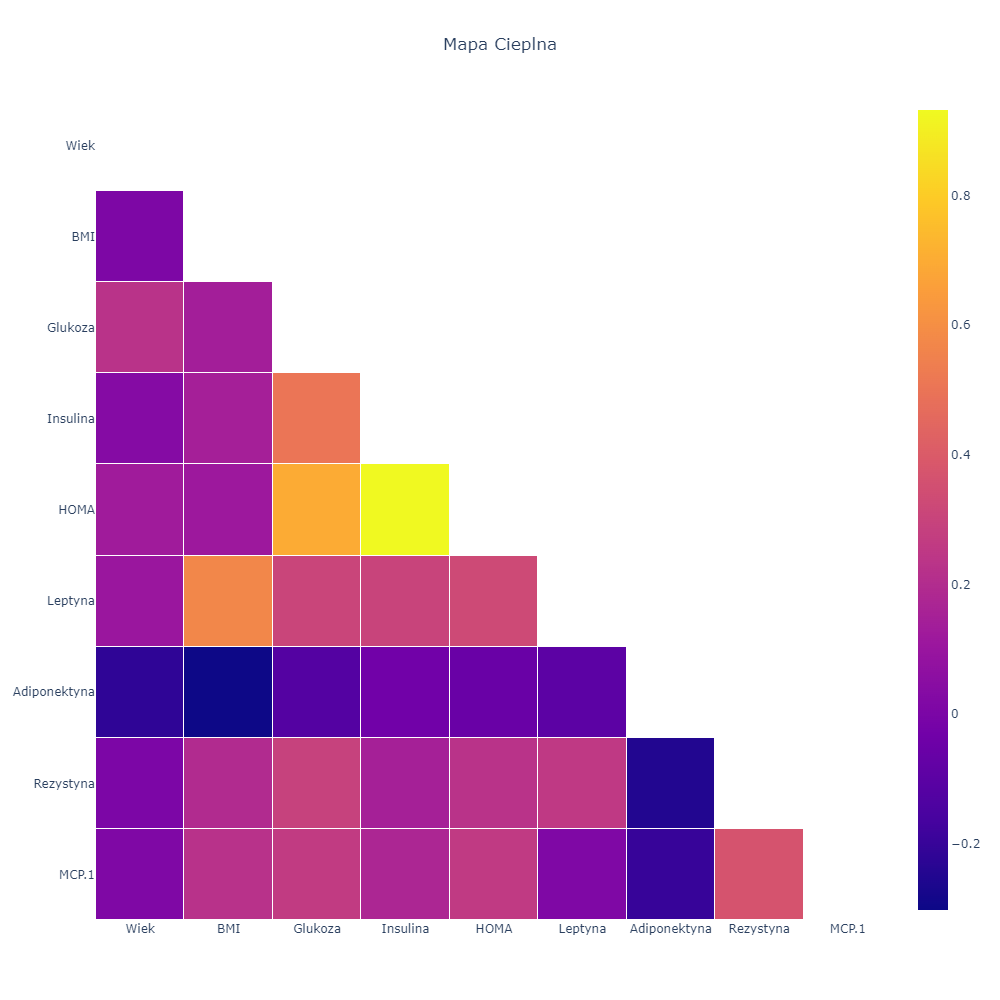
\includegraphics[scale=0.3]{heatNOCODE.png}
\caption{Mapa cieplna}
\end{figure}

Poszczególne segmenty mapy z rys. 4.7 reprezentują korelacje między dwiema zmiennymi, im kolor jest jaśniejszy tym bardziej dane są skorelowane. Na wykresie można wyraźnie zaobserwować bardzo wysoką korelację między cechami HOMA a insuliną, rzędu 0.93. Na podstawie tej informacji można zdecydować czy nie korzystnej będzie pozbycie się jednej z tych cech gdyż niosą praktycznie tę samą informację. Zważając charakter cech zbioru oraz ich małą ilość, jak również mały rozmiar samego zbioru zdecydowałem się zachować obydwie te cechy, bez żadnych zmian. Należy również wspomnieć, iż mapa cieplna zazwyczaj jest odbita lustrzanie po przekątnej, lecz w zaprezentowanym przykładnie górne odbicie zostało „zamaskowane”, w celu zwiększenia przejrzystości wykresu. Po wykonanej analizie, można dojść do wniosków że podział pacjentek na podstawie obecnych danych może okazać się problematyczny. Żadna z cech nie rozdziela danych w jednoznaczny sposób, oraz wiele z wyników pokrywa się ze sobą zarówno dla tych zdrowych, jak i chorych osób.

\section{Dopasowanie modeli}

Po wykonanej analizie można przystąpić do przygotowania zbioru danych do dopasowania modeli uczenia maszynowego. W pierwszej kolejności skupiłem się na wartościach odstających, w przypadku których istnieją dwie opcje: po pierwsze, najprostsze usunięcie rekordów zawierających te wartości, po drugie „przycięcie” czyli odpowiednie ich zmniejszenie lub zwiększenie tak aby przyjmowały wartości mniej skrajne. Z powodu małego rozmiaru zbioru zdecydowałem się na drugą opcję. Do zidentyfikowania wartości odstających użyję przedziału międzykwartylowego, czyli różnicy między pierwszym a trzecim kwartylem. Poniżej przedstawiono schemat „przycinania” wartości odstających oraz kod wykonujący tę operację [23]:

\begin{enumerate}
    \item Oblicz przedział międzykwartylowy \textit{ }$IQR=Q_3-Q_1$\textit{.}
    \item Oblicz wartości minimalną i maksymalną do jakiej będą przyrównywane odnalezione wartości odstające odpowiednio ${min =Q_1-1.5*IQR\ }$ oraz ${max =Q_3+1.5*IQR\ }$.
    \item Jeśli wartość nie znajduję się w przedziale $\left\langle min,max\right\rangle $ zastąp ją odpowiednio wartości $min$ lub $max$.
\end{enumerate}

\begin{lstlisting}[language=Python, caption='Przycinanie' wartości odstających]
q1 = df.quantile(0.25)
q3 = df.quantile(0.75)
iqr = q3 - q1
min_Wart_kwartyl = q1 - 1.5 * iqr
max_Wart_kwartyl = q3 + 1.5 * iqr
df_wartosci_przyciete = df.drop(columns=['Klasyfikacja', 'Wiek', 'PrzedzialWiekowy'])
for col in df_wartosci_przyciete.columns:
    for val in range(len(df_wartosci_przyciete[col])):
                     if df_wartosci_przyciete[col][val] < min_Wart_kwartyl[col]: df_wartosci_przyciete[col][val] = min_Wart_kwartyl[col]
                     if df_wartosci_przyciete[col][val] > max_Wart_kwartyl[col]: df_wartosci_przyciete[col][val] = max_Wart_kwartyl[col]
df_wartosci_przyciete.insert(0, 'Wiek', df['Wiek'])
df_wartosci_przyciete.insert(0, 'Klasyfikacja', df['Klasyfikacja'])
df_wartosci_przyciete['Klasyfikacja'].replace({'Zdrowa': 0, 'Chora': 1}, inplace=True)
\end{lstlisting}

Kod poza przycinaniem wartości odstających ze wszystkich cech numerycznych poza cechą „Wiek” usuwa stworzoną cechę „PrzedziałWiekowy” oraz zamienia wartości cechy „Klasyfikacja” ze „Zdrowa” i „Chora” na 0 i 1.\\
Następnym krokiem jest podział zbioru na zbiory treningowe oraz testowe. W tym celu najpierw podzieliłem zbiór na podzbiory x, czyli zbiór zawierający atrybuty na podstawie których przewidywane będą etykiety znajdujące się w zbiorze y. Następnie wykorzystałem metodę \textit{scikit-learn.model\_selection.train\_test\_split}. Wielkość zbioru testowego można regulować za pomocą hiperparametru \textit{test\_size}, który w moim przypadku wynosi 0.2, czyli 20\% danych będą to dane testowe. Zbiory wejściowe zostaną poddane standaryzacji za pomocą funkcji \textit{sklearn.preprocessing.StandardScaler}. Skaluje ona dane do standardowej dystrybucji normalnej (ang. Standard Normal Distribution, SND), czyli wszystkie dane zostają przeskalowane tak aby ich średnia wynosiła 0, a odchylenie standardowe 1.

\begin{lstlisting}[language=Python, caption=Przygotowanie zbiotów treningowych oraz testowych]
x = df_wartosci_przyciete.drop('Klasyfikacja', axis=1)
y = df_wartosci_przyciete['Klasyfikacja']
x_train, x_test, y_train, y_test = train_test_split(x, y, test_size=0.2, random_state=42)
scaler = StandardScaler()
x_train = scaler.fit_transform(x_train)
x_test = scaler.fit_transform(x_test)
\end{lstlisting}


Po wykonaniu tychże czynności, można przystąpić do inicjalizacji i dopasowania modeli do danych. Poniżej przedstawiony kod wykonuje te operacje inicjalizując kolejno model lasów losowych, K-najbliższych sąsiadów (KNN), AdaBoost oraz model stackingu, który jako model poziomu pierwszego wykorzystuje wcześniej zainicjalizowane modele, zaś funkcje meta modelu pełni regresja logistyczna. Modele są dopasowywane za pomocą funkcji \textit{fit}, którą posiada każdy model z biblioteki scikit-learn, a następnie predykcje wykonane przez modele zapisane zostają do oddzielnych zmiennych i posłużą one do oceny jakości modeli.

\newpage

\begin{lstlisting}[language=Python, caption=Dopasowanie modeli]
Las_Losowy = RandomForestClassifier(n_estimators=100, random_state=42)
KNN = KNeighborsClassifier(n_neighbors=10, weights='distance')
AdaBoost = AdaBoostClassifier(n_estimators=100, random_state=42)   
lista_modeli = [
    ('Las Losowy', Las_Losowy),
    ('AdaBoost', AdaBoost),
    ('KNN', KNN)
]
Stacking = StackingClassifier(estimators= lista_modeli, final_estimator=LogisticRegression())
Las_Losowy.fit(x_train, y_train)
KNN.fit(x_train, y_train)
AdaBoost.fit(x_train, y_train)
Stacking.fit(x_train, y_train)
Las_Losowy_Predykcje = Las_Losowy.predict(x_test)
KNN_Predykcje = KNN.predict(x_test)
AdaBoost_Predykcje = AdaBoost.predict(x_test)
Stacking_Predykcje = Stacking.predict(x_test)
\end{lstlisting}


\chapter{Ocena modeli}
Istnieje wiele sposobów oceny modelu uczenia maszynowego, z których każdy niesie ważną informację, na podstawie której można dokonać wyboru odpowiedniego modelu dla przeznaczonego mu zadania. Aby zrozumieć odpowiednie metryki należy zaznaczyć że wykorzystują one pojęcia dwóch typów błędu [24]:\\
\textbf{Błąd typu pierwszego (FP)} – odrzucenie hipotezy fałszywości (ang. null hypothesis, False Positive), występuje wtedy gdy wynik jest fałszywie pozytywny.\\
\textbf{Błąd typu drugiego (FN)} – odrzucenie hipotezy prawdziwości (ang. False Negative), odwrotność typu pierwszego, występuje gdy wynik jest fałszywie negatywny.\\
Nie istnieje idealna metryka wydajności modelu ukazująca wszystkie jego wady i zalety, dlatego też zawsze należy brać pod uwagę wszystkie metryki i na tej podstawie dokonywać wyboru w sposób całościowy.

\section{Macierz pomyłek}
Macierz pomyłek (ang. confusion matrix) w przejrzysty sposób przedstawia zależności między błędami predykcji danego modelu uczenia maszynowego. Na rysunku 5.1 przedstawiona została ilustracja macierzy pomyłek dla problemu predykcji złośliwości raka.

\begin{figure}[H]
\centering
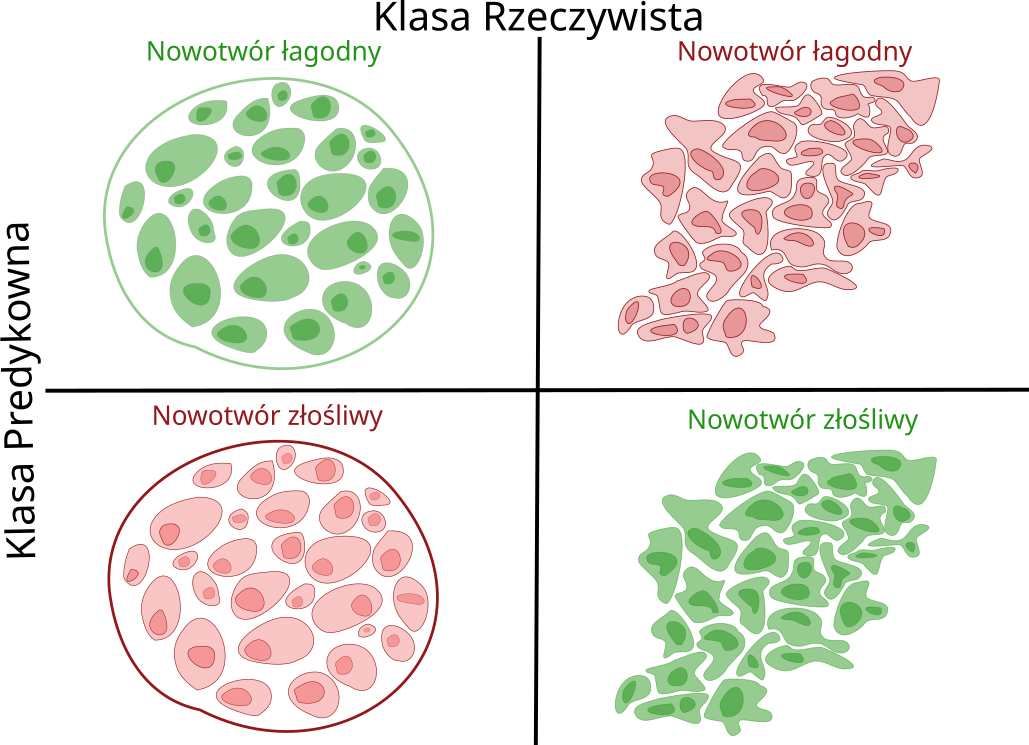
\includegraphics[scale=0.5]{confMat.png}
\caption{Schemat macierzy pomyłek dla klasyfikacji nowotworu}
\end{figure}

Klasyfikacja nowotworu jest przykładem problemu klasyfikacji binarnej, przez co macierz składać się będzie z dwóch kolumn i wierszy. Kolumny przedstawiają wartości rzeczywiste, wiersze zaś wartości predykowane. Błędy typu pierwszego znajdują się w prawym górnym rogu, zaś typu drugiego w lewym dolnym rogu, natomiast przekątna macierzy składa się z predykcji poprawnych. Macierz pomyłek może również być stworzona na tej samej zasadzie dla problemów klasyfikacji z większą ilością klas. Listing 5.1 zawiera kod wykorzystujący wspomnianą wcześniej mapę cieplną do stworzenia macierzy pomyłek rysunek 5.2 natomiast przedstawia oznaczoną macierz pomyłek.


\begin{lstlisting}[language=Python, caption=Funkcja tworząca macierz pomyłek]
def macierz_pomylek(tytul, y_test, y_pred):
    fig = ff.create_annotated_heatmap(metrics.confusion_matrix(y_test, y_pred), colorscale='Greens')
    fig.add_annotation(dict(font=dict(color="black",size=20), x=0.5, y=1.10,
                            showarrow=False, text="Klasa Predykowana", xref="paper", yref="paper"))
    fig.add_annotation(dict(font=dict(color="black",size=20), x=-0.10, y=0.5,
                            showarrow=False, text="Klasa Rzeczywista", textangle=-90, xref="paper", yref="paper"))
    fig.update_yaxes(autorange="reversed")
    fig.update_layout(width = 500, height = 500, title_text = tytul)
    fig.show()
\end{lstlisting}

\begin{figure}[H]
\centering
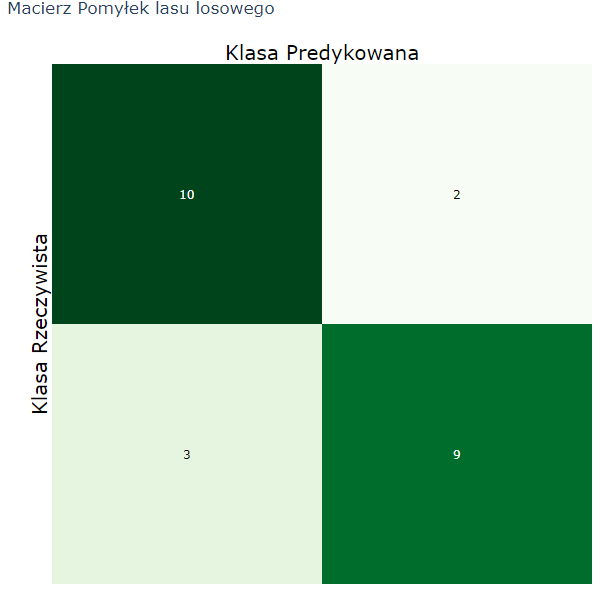
\includegraphics[scale=0.6]{pxConfMat.png}
\caption{Postać liczbowa macierzy pomyłek}
\end{figure}

\section{Precyzja i czułość}
Kolejnymi metodami oceny modelu uczenia maszynowego są Precyzja oraz Czułość. Obydwie te metryki wykorzystują błędy typu pierwszego (FP) oraz drugiego (FN), wraz z ich odwrotnościami czyli True Positives (TP) oraz True Negatives (TN), aby zobrazować relacje między typami błędów popełnianych przez dany model.\\
Precyzja jest funkcją FP i FP i obrazuje jak precyzyjny jest nasz model, czyli na ile procent możemy być pewni poprawności wyniku modelu. Jest ona opisana wzorem [25]:\\

\begin{equation}
Precyzja=\ \frac{TP}{TP+FP}
\end{equation}


Oznacza to że gdy współczynnik precyzji wynosi 0.81, (jak dla wcześniej wspomnianego modelu lasu losowego) możemy być na 80\% pewni że przewidywany wynik jest prawdziwy.
Czułość natomiast jest funkcją TP i FN i obrazuje jaki procent rekordów został pozytywnie zaklasyfikowany. Jest ona opisana wzorem [25]:

\begin{equation}
Czu\textrm{\l}o\textrm{\'{s}}\textrm{\'{c}}=\ \frac{TP}{TP+FN}    
\end{equation}


Współczynnik ten dla modelu lasu losowego jest równy 0.75, co oznacza że 75\% chorych zostało poprawnie zaklasyfikowanych.
Przy dostrajaniu, lub samym wyborze musimy uwzględnić kompromis między precyzją a czułością (ang. precision/recall tradeoff), wartości te są odwrotnie skorelowane - wraz z wzrostem precyzji czułość naszego algorytmu spada, i odwrotnie. Decyzja podejmowana jest głównie na podstawie istotności pojedynczych predykcji, np. gdyby potencjalny model miałby decydować o tym czy pacjentka rozpoczyna leczenie nowotworu, ważniejsza byłaby precyzja, gdyż konsekwencje pomyłki są znacznie większe niż gdyby funkcją klasyfikatora było wyróżnienie pacjentek poddanych dalszym badaniom - wtedy moglibyśmy się skupić na czułości, ponieważ zależałoby nam aby przebadać jak najwięcej potencjalnych chorych, nawet jeśli dalsze badania miały wykazać iż są zdrowi.


\section{Dokładność i wynik F1}

Posiadanie wielu metryk do oceny czegokolwiek może okazać się nie wygodne i mylące, tak samo jest z algorytmami uczenia maszynowego. W tym celu określone zostały dwie metryki mające na celu ujednolicenie określania jakości danego modelu. Pierwszą z nich jest Dokładność, najprostsza i najbardziej oczywista miara jakości algorytmu. Jest ona niczym więcej niż procentem poprawnie sklasyfikowanych rekordów z całego zbioru i opisana jest równaniem [25]:

\begin{equation}
Dok\textrm{\l}adno\textrm{\'{s}}\textrm{\'{c}}=\ \frac{TP+TN}{TP+FP+TN+FN}    
\end{equation}


Jest to niestety metryka bardzo wrażliwa na strukturę samego zbioru danych, jest ona idealna gdy nasz zbiór jest zbalansowany (tyle samo przykładów dla każdej z klas).\\
Zbiór danych Breast Cancer Coimbra składa się z rekordów 64 chorych i 52 zdrowych pacjentek, oznacza to że gdyby algorytm uczenia maszynowego po prostu uznawał każdą pacjentkę za chorą uzyskał on by wynik 55\% dokładności, co oznacza że dokładność jest dobrą metryką w przypadku tego zbioru. Gdyby natomiast zbiór nasz składał się ze 100 chorych pacjentek i 16 zdrowych ten sam algorytm uzyskałby wynik 86\% dokładności, co może być mylące.
Metryką próbującą rozwiązać ten problem jest Wynik \textit{F1}. Wynik ten jest niczym innym jak średnią harmoniczną wartości precyzji i czułości i dany jest wzorem [25]:

\begin{equation}
Wynik\ F1=\frac{2}{Precyzja^{-1}*Czu\textrm{\l}o\textrm{\'{s}}{\textrm{\'{c}}}^{-1}}=2*\frac{Precyzja*Czu\textrm{\l}o\textrm{\'{s}}\textrm{\'{c}}}{Precyzja+Czu\textrm{\l}o\textrm{\'{s}}\textrm{\'{c}}}    
\end{equation}


Wykorzystując tylko rodzaje poprawnych i błędnych klasyfikacji wynik F1 można opisać zależnością [25]:

\begin{equation}
Wynik\ F1=\ \frac{TP}{TP+\ \frac{FP+FN}{2}}    
\end{equation}


Istnieje również wariant wyniku \textit{F1} biorący pod uwagę o ile ważniejsza (lub mniej ważna) jest czułość algorytmu od jego precyzji. Nosi on nazwę wyniku $F_{\beta }$ gdzie beta jest wskaźnikiem istotności czułości. Opisany jest on wzorem [25]:

\begin{equation}
Wynik\ F_{\beta }=\left(1+{\beta }^2\right)*\frac{Precyzja*Czu\textrm{\l}o\textrm{\'{s}}\textrm{\'{c}}}{\left({\beta }^2*P\textrm{�}\textrm{�}ecyzja\right)+Czu\textrm{\l}o\textrm{\'{s}}\textrm{\'{c}}}
\end{equation}


Poniżej przedstawiony został kod obliczający i wypisujący wartości wszystkich wspomnianych wcześniej metryk oraz przykładowe wyjście dla lasu losowego. Funkcja ponadto zapisuje obliczone wyniki do tablicy „metryki” na potrzeby narysowania wykresu ułatwiającego porównanie wszystkich modeli.

\begin{lstlisting}[language=Python, caption=Funkcja wypisująca i zapisująca metryki]
metryki = []
def wypisz_metryki(model_name, y_test, y_pred):
    print("\nMetryki dla modelu: " + str(model_name))
    print("Dokladnosc: ",metrics.accuracy_score(y_test, y_pred))
    print("Precyzja: ",metrics.precision_score(y_test, y_pred))
    print("Czulosc: ",metrics.recall_score(y_test, y_pred))
    print("Wynik F1: ",metrics.f1_score(y_test, y_pred))
    metryki.append([model_name, metrics.accuracy_score(y_test, y_pred), metrics.precision_score(y_test, y_pred),
                          metrics.recall_score(y_test, y_pred), metrics.f1_score(y_test, y_pred)])
\end{lstlisting}

\begin{figure}[H]
\centering
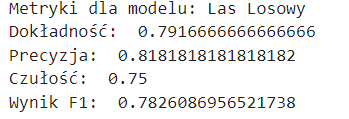
\includegraphics[scale=0.6]{wypisz_metrykiShow.png}
\end{figure}

Następnie tabela „metryki” zostaje zamieniona na obiekt \textit{DataFrame}, dzięki czemu w łatwy sposób można stworzyć wykres porównujący wszystkie modele (rys. 5.3):

\begin{lstlisting}[language=Python, caption=Tworzenie wykresu słupkowego porównującego modele]
metryki = pd.DataFrame(metryki, columns = ['Model', 'Dokladnosc', 'Precyzja', 'Czulosc', 'Wynik F1'])
fig = go.Figure()
fig.add_trace(go.Histogram(histfunc="sum", x=metryki['Model'], y=metryki['Dokladnosc'], name='Dokladnosc'))
fig.add_trace(go.Histogram(histfunc="sum", x=metryki['Model'], y=metryki['Precyzja'], name='Precyzja'))
fig.add_trace(go.Histogram(histfunc="sum", x=metryki['Model'], y=metryki['Czulosc'], name='Czulosc'))
fig.add_trace(go.Histogram(histfunc="sum", x=metryki['Model'], y=metryki['Wynik F1'], name='Wynik F1'))
fig.update_layout(bargap=0.2, bargroupgap=0.1, height = 500, width = 800)
\end{lstlisting}

\begin{figure}[H]
\centering
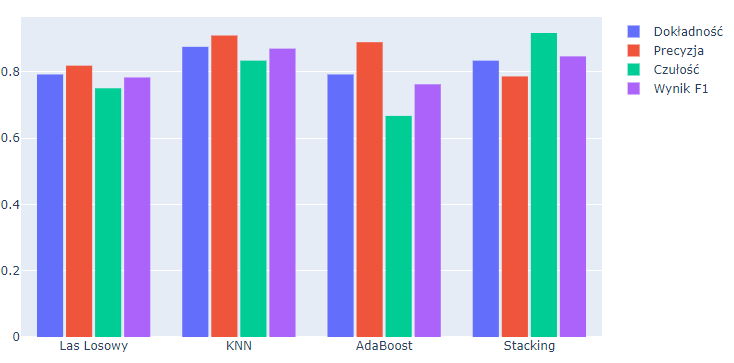
\includegraphics[scale=0.5]{metrykiHistShow.png}
\caption{Porównanie modeli ze względu na Dokładność, Precyzję, Czułość oraz Wynik F1}
\end{figure}

Jak widać z wykresu najlepszym ogólnym klasyfikatorem okazał się model KNN, z wynikiem dokładności rzędu 87.5\% oraz precyzji na poziomie 90\%. Tuż za nim był model stackingu, który lepszy okazał się tylko pod względem czułości rzędu 91,6\%. Biorąc pod uwagę zarówno wielkość jak i charakter zbioru danych nie są to wyniki złe, lecz w przypadku zamiaru wykorzystania modeli poza sferą badawczą na pewno pozostawiają trochę do życzenia.

\chapter{Wnioski}
Analizując dane uzyskane na podstawie prezentowanych algorytmów, można stwierdzić że diagnostyka chorób nowotworowych nie jest aż tak skomplikowanym zadaniem, wyniki rzędu 87.5\% mogą wydawać się wysokie, lecz biorąc pod uwagę to że, w przeciwieństwie do wielu innych zastosowań uczenia maszynowego, w grę wchodzi ludzkie zdrowie, a nawet życie, nie wskazanym byłoby formułowanie żądnych decyzji tylko na podstawie tychże algorytmów.
Zdecydowaną zaletą analizowanego zbioru danych jest to, że wykorzystuje on badania krwi do pozyskania informacji na bazie których można przewidywać występowanie chorób nowotworowych. Badania te są bardzo mało inwazyjne i często wykonywane, przez co każda potencjalna pacjentka mogłaby skorzystać z modelu predykcyjnego nijako „przy okazji” innych badań. W tym przypadku potencjalny model powinien skupiać się na metryce \textit{Czułości}. Praktyka taka mogłaby potencjalnie zwiększyć ilość pacjentek decydujących się na dalsze badania, co mogłoby skutkować spadkiem śmiertelności osób cierpiących na choroby nowotworowe, ponieważ mimo wielu innowacyjnych metod leczenia, nadal najlepszym lekarstwem na raka jest jego wczesne wykrycie.\\
Modele uczenia maszynowego, można również potraktować jako swoistą pomoc dla lekarza, lub nawet (wychodząc poza sferę uczenia maszynowego do obszaru samej sztucznej inteligencji) tworzyć personalnych asystentów, służących lekarzom swoją wiedzą. Podejście to mogłoby efektywnie wyeliminować jeden z większych problemów zastosowania zarówno ucznia maszynowego jak i sztucznej inteligencji w medycynie - mianowicie braku zaufania ludzi do maszyn, zwłaszcza w przedziałach wiekowych najbardziej narażonych na wystąpienie nowotworu.


\listoffigures{}


\lstlistoflistings{}

\markboth{}{}


\chapter*{Bibliografia}
\addcontentsline{toc}{chapter}{Bibliografia}

\thispagestyle{empty}
[1] Pranav Rajpurkar, Jeremy Irvin, Kaylie Zhu, Brandon Yang, Hershel Mehta, Tony Duan, Daisy Ding, Aarti Bagul, Curtis Langlotz, Katie Shpanskaya, Matthew P. Lungren, Andrew Y. Ng,\\
CheXNet: Radiologist-Level Pneumonia Detection on Chest X-Rays with Deep Learning, https://stanfordmlgroup.github.io/projects/chexnet/ (data dostępu 19.04.2022)\\

[2] Angelika Janowicz,  Agnieszka Widera, Rodzaje nowotworów łagodnych i złośliwych,\\ \url{https://www.welbi.pl/jakie-sa-rodzaje-nowotworow-co-warto-wiedziec/} (aktualizacja: 18.01.2022)\\

[3] Tomasz Jastrzębski, Kancerogeneza – czyli jak powstaje rak i dlaczego\\ \url{https://www.onkonet.pl/dp_kancerogeneza.php#:~:text=Terminem\%20\%E2\%80\%9Ekancerogeneza\%E2\%80\%9D\%2C\%20\%E2\%80\%9Ekarcinogeneza,nawet\%2010\%20lat\%20i\%20wi\%C4\%99cej/}  Serwis onkologiczny (data dostępu 19.04.2022)\\

[4] Nowotwory – wprowadzenie,  \url{http://onkologia.org.pl/nowotwory-wprowadzenie/ Krajowy rejestr nowotworów} (data dostępu 19.04.2022)\\

[5] Metody leczenia nowotworów,\url{https://alivia.org.pl/wiedza-o-raku/metody-leczenia-nowotworow/} Onkofundacja Alivia (data dostępu 19.04.2022)\\

[6] National Cancer Institute, Immunotherapy to Treat Cancer,
\url{https://www.cancer.gov/about-cancer/treatment/types/immunotherapy#:~:text=Immunotherapy\%20is\%20a\%20type\%20of,a\%20type\%20of\%20biological\%20therapy} (aktualizacja: 24.09.2019)\\

[7] Czym jest hormonoterapia nowotworów?, \url{https://alivia.org.pl/wiedza-o-raku/czym-jest-hormonoterapia-nowotworow/}  Onkofundacja Alivia (data dostępu 22.04.2022)\\

[8] Arthur L. Samuel, Some Studies in Machine Learning Using the Game of Checkers, IBM Journal of Research and Development, 44:1.2, (1959): 210\\

[9] Frank Rosenblatt, The perceptron: A probabilistic model for information storage and organization in the brain, Psychological Review, Vol. 65, (1958) No. 6: 386\\

[10] Keith D. Foote, A Brief History of Machine Learning, \url{https://www.dataversity.net/a-brief-history-of-machine-learning/} (data dostępu 22.03.2022)\\

[11] Peter Brouce, Andrew Brouce, Peter Gedeck, Practical Statistics for Data Scientists: 50+ Essential Concepts Using R and Python, O’Raily (2020), wydanie polskie Statystyka praktyczna w data science: 50 kluczowych zagadnień w językach R i Python, Helion (2021)\\

[12] Robert E. Shapire, The strength of weak learnability, Machine Learning, 5, (1990): 197\\

[13] Jürgen Schmidhuber, Sepp Hochreiter, Long short-term memory, Neural Computation, 9:8, (1997): 1735.\\

[14] Aurélien Géron. Hands-on Machine Learning with Scikit-Learn, Keras, and TensorFlow: Concepts, Tools, and Techniques to Build Intelligent\\ Systems, 2nd Edition, O’Raily (2020)\\

[15] Cztery typy uczenia maszynowego, \url{https://www.sas.com/pl_pl/news/informacje-prasowe-pl/2018/cztery-typy-uczenia-maszynowego.html} (data dostępu 22.03.2022)\\

[16] Decision tree learning, \url{https://en.wikipedia.org/wiki/Decision_tree_learning},  (data dostępu 22.03.2022)\\

[17] Robert E. Schapire, Explaining AdaBoost \url{http://rob.schapire.net/papers/explaining-adaboost.pdf}  (data dostępu 22.04.2022)\\

[18] Jason Brownlee, Stacking Ensemble Machine Learning With Python,\\ 
\url{https://machinelearningmastery.com/stacking-ensemble-machine-learning-with-python/}\\
(data dostępu 23.04.2022)\\

[19] Charu C. Aggarwal, Data Classification Algorithms and Applications, Chapman and Hall/CRC (2020)\\

[20] Sarang Anil Gokte, Most Popular Distance Metrics Used in KNN and When to Use Them\\ \url{https://www.kdnuggets.com/2020/11/most-popular-distance-metrics-knn.html}\\ 
(data dostępu 23.04.2022)\\

[21] Machine Learning Repository, Breast Cancer Coimbra Data set,\\
 \url{https://archive.ics.uci.edu/ml/datasets/Breast+Cancer+Coimbra} (data dostępu 23.04.2022)\\

[22] McKinney Wes, Python for Data Analysis: Data Wrangling with Pandas, NumPy, and IPython, O’Raily (2018), wydanie polskie Python w analizie\\ danych. Przetwarzanie danych za pomocą pakietów Pandas i NumPy oraz środowiska Ipython (2018)\\

[23] How to Find Outliers Using the Interquartile Range, \url{https://www.statology.org/find-outliers-with-iqr/} (data dostępu 23.04.2022)\\

[24] Machine Learning Crash Course, Classification: True vs. False and Positive vs. Negative,\\
\url{https://developers.google.com/machine-learning/crash-course/classification/true-false-positive-negative} (data dostępu 23.04.2022)\\

[25] Thomas Wood, F-Score,\newline \url{https://deepai.org/machine-learning-glossary-and-terms/f-score} (data dostępu 23.04.2022)\\



\end{document}